%%%%%%%%%%%%%%%%%%%%%%%%%%%%%%%%%%%%%%%%%%%%%%%%%%%%%%%
%%%%               FORMATTING AND COLORING         %%%%
%%%%%%%%%%%%%%%%%%%%%%%%%%%%%%%%%%%%%%%%%%%%%%%%%%%%%%%
\documentclass[xcolor=dvipsnames]{beamer}

\definecolor{Fuchsia}{HTML}{49796b}
\definecolor{SlateGrey}{HTML}{003800}
\definecolor{FuchsiaDark}{HTML}{305047}

%\definecolor{LightGrey}{HTML}{666666}

\colorlet{accent}{Fuchsia}
\colorlet{emphasis}{SlateGrey}

\usepackage{caption}

\usetheme{CambridgeUS}
\useinnertheme{rectangles}
\useoutertheme{infolines}

%%%%%%%%%%%%%%%%%%%%%%%%%%%%%%%%%%%%%%%%%%%%%
%this adds in the circles to the right of background
%%%%%%%%%%%%%%%%%%%%%%%%%%%%%%%%%%%%%%%%%%%%%
\makeatletter
\def\insertsubsectionnavigationhorizontal#1#2#3{%
    \hbox to #1{{%
        \usebeamerfont{subsection in head/foot}\usebeamercolor[fg]{subsection in head/foot}
        \beamer@currentsubsection=0%
        \def\sectionentry##1##2##3##4##5{}%
        \def\slideentry##1##2##3##4##5##6{\ifnum##6=\c@part\ifnum##1=\c@section%
      \ifnum##2>\beamer@currentsubsection%
      \box\beamer@sectionbox\hskip1.875ex plus1fill%
            \hbox to 0pt{%
                    \global\beamer@section@min@dim\beamer@tempdim
                        \beamer@link(##4){%
                            \usebeamerfont{mini frame}%
                            \ifnum\c@section=##1%
                                \ifnum\c@subsection=##2%
                                    \usebeamercolor[fg]{mini frame}%
                                    \ifnum\c@subsectionslide=##3%
                                        \usebeamertemplate{mini frame}%\beamer@minislidehilight%
                                    \else%
                                        \usebeamertemplate{mini frame in current subsection}%\beamer@minisliderowhilight%
                                    \fi%
                                \else%
                                    \usebeamercolor{mini frame}%
                                    %\color{fg!50!bg}%
                                    \usebeamertemplate{mini frame in other subsection}%\beamer@minislide%
                                \fi%
                            \else%
                                \usebeamercolor{mini frame}%
                                                                %\color{fg!50!bg}%
                                \usebeamertemplate{mini frame in other subsection}%\beamer@minislide%
                            \fi%
                        }%
                \hskip-10cm plus 1fil%
            }%
            \fi\fi\fi\ignorespaces
        }%
        #2\hskip.3cm\setbox\beamer@sectionbox=\hbox{}%
        \hskip-1.875ex plus-1fill\dohead%
        \box\beamer@sectionbox\hfil\hskip.3cm%
        #3
    }}
}

\setbeamertemplate{footline}%{infolines theme}
{
  \leavevmode%
  \hbox{%
  \begin{beamercolorbox}[wd=.333333\paperwidth,ht=2.25ex,dp=1ex,center]{author in head/foot}%
    \usebeamerfont{author in head/foot}\insertshortauthor\expandafter\beamer@ifempty\expandafter{\beamer@shortinstitute}{}{~~(\insertshortinstitute)}
  \end{beamercolorbox}%
  \begin{beamercolorbox}[wd=.333333\paperwidth,ht=2.25ex,dp=1ex,center]{title in head/foot}%
    \usebeamerfont{title in head/foot}\insertshorttitle
  \end{beamercolorbox}%
  \begin{beamercolorbox}[wd=.333333\paperwidth,ht=2.25ex,dp=1ex,right]{date in head/foot}%
    \usebeamerfont{date in head/foot} %\insertshortdate{} % remove the date from each slide 
    % could insert text here to make it display in the footer 
    \hspace*{2em}
    \insertframenumber{} / \inserttotalframenumber\hspace*{2ex} 
  \end{beamercolorbox}}%
  \vskip0pt%
}
\makeatother

\setbeamertemplate{headline}
{
  \leavevmode%
  \hbox{%
  \begin{beamercolorbox}[wd=.5\paperwidth,ht=2.65ex,dp=1.5ex,right]{section in head/foot}%
    \usebeamerfont{section in head/foot}\bfseries\insertsectionhead\hspace*{2ex}
  \end{beamercolorbox}%
  \begin{beamercolorbox}[wd=.5\paperwidth,ht=2.65ex,dp=1.5ex,left]{subsection in head/foot}%
    \usebeamerfont{subsection in head/foot}\setbeamercolor{section in head/foot}{fg=Fuchsia!125,bg=white}
    \vspace*{.01cm}\insertsubsectionnavigationhorizontal{.5cm}{\hskip-.1cm}{}
  \end{beamercolorbox}}%
  \vskip0pt%
}
% gets rid of navigation symbols
\setbeamertemplate{navigation symbols}{}
% add figures numbering
\setbeamertemplate{caption}[numbered]

\setbeamercolor{frametitle}{fg=Fuchsia,bg=Fuchsia!20}
\setbeamercolor{section in head/foot}{fg= SlateGrey!20, bg=Fuchsia}
\setbeamercolor{title in head/foot}{fg=Fuchsia}
\setbeamercolor{subsection in head/foot}{fg=Fuchsia}
\setbeamercolor{author in head/foot}{bg=Fuchsia, fg=Fuchsia}
\setbeamercolor{date in head/foot}{fg=Fuchsia}
\setbeamercolor{structure}{fg=Fuchsia, bg= SlateGrey}
\setbeamercolor{frametitle}{fg= Fuchsia}
\setbeamercolor{title}{fg=Fuchsia}
\setbeamercolor*{palette tertiary}{bg=Fuchsia}
\setbeamercolor{section in sidebar}{fg=Fuchsia}
\setbeamercolor{titlelike}{bg =SlateGrey!5}

%%%%%%%%%%%%%%%%%%%%%%%%%%%%%%%%%%%%%%%%%%%%%%%%%%%
% End of customizing the theme layout and colors 
%%%%%%%%%%%%%%%%%%%%%%%%%%%%%%%%%%%%%%%%%%%%%%%%%%%
\usepackage{comment}
\usepackage[T1]{fontenc}
\usepackage[default]{lato}
\usepackage[english]{babel}
\usepackage[utf8x]{inputenc}
\usepackage{pslatex}
\usepackage{fontawesome}
\usepackage{animate}

\usepackage{xmpmulti}

\usepackage{subcaption}
\captionsetup{compatibility=false}
%%%%%%%%%%%%%%%%%%%%%%%%%%%%%%%%%%%%%%%%%%%%%%%%%%%%%%%
%%%%%%%%%%%%%%%%%%%%%%%%%%%%%%%%%%%%%%%%%%%%%%%%%%%%%%%
%%%%          Beginning of the slide deck          %%%%
%%%%%%%%%%%%%%%%%%%%%%%%%%%%%%%%%%%%%%%%%%%%%%%%%%%%%%%
%%%%%%%%%%%%%%%%%%%%%%%%%%%%%%%%%%%%%%%%%%%%%%%%%%%%%%%

\definecolor{climateChange}{HTML}{F8766D}
\definecolor{recentTrends}{HTML}{00BFC4}
\definecolor{activeGreen}{HTML}{00cc00}
\definecolor{fuelBreakColor}{HTML}{70AD47}
\definecolor{salvageLogColor}{HTML}{0099FF}
\definecolor{fuelReductionColor}{HTML}{EB45BC}


\newenvironment{a2env}{\only{\setbeamercolor{local structure}{fg=climateChange}}}{}
\newenvironment{rtenv}{\only{\setbeamercolor{local structure}{fg=recentTrends}}}{}
%%%%%%%%%%%%
%title page%
%%%%%%%%%%%%
\title[Yellowstone Visitor Trends]{Time Series Analysis Project:\\ Yellowstone Visitor Trends}
\author{Michael Dunn, Jacob Klein, and Evan Waldmann}
\institute{University of Central Florida}
\date{\scriptsize{April 18th, 2019}}

\begin{document}
\begin{frame}
  \titlepage
  \vfill

\end{frame}

\section{Background}


% Uncomment these lines for an automatically generated outline.
%\begin{frame}{Outline}
%  \tableofcontents
%\end{frame}


%%%%%%%%%%%%%%%%%%%%%%%%%%%
%beginning of actual sides%
%%%%%%%%%%%%%%%%%%%%%%%%%%%
\subsection{}


\section{General Trends}
\subsection{}

\begin{frame}{Yellowstone visitor attendance 1986-2017}
%
%\begin{itemize}
%\item With the intent of forecasting the number of visitors the park attracts each year, we set out on this project to analyze and fit a model to this time series of the number of visits to the park each month. 
%\end{itemize}
\begin{figure}
\centering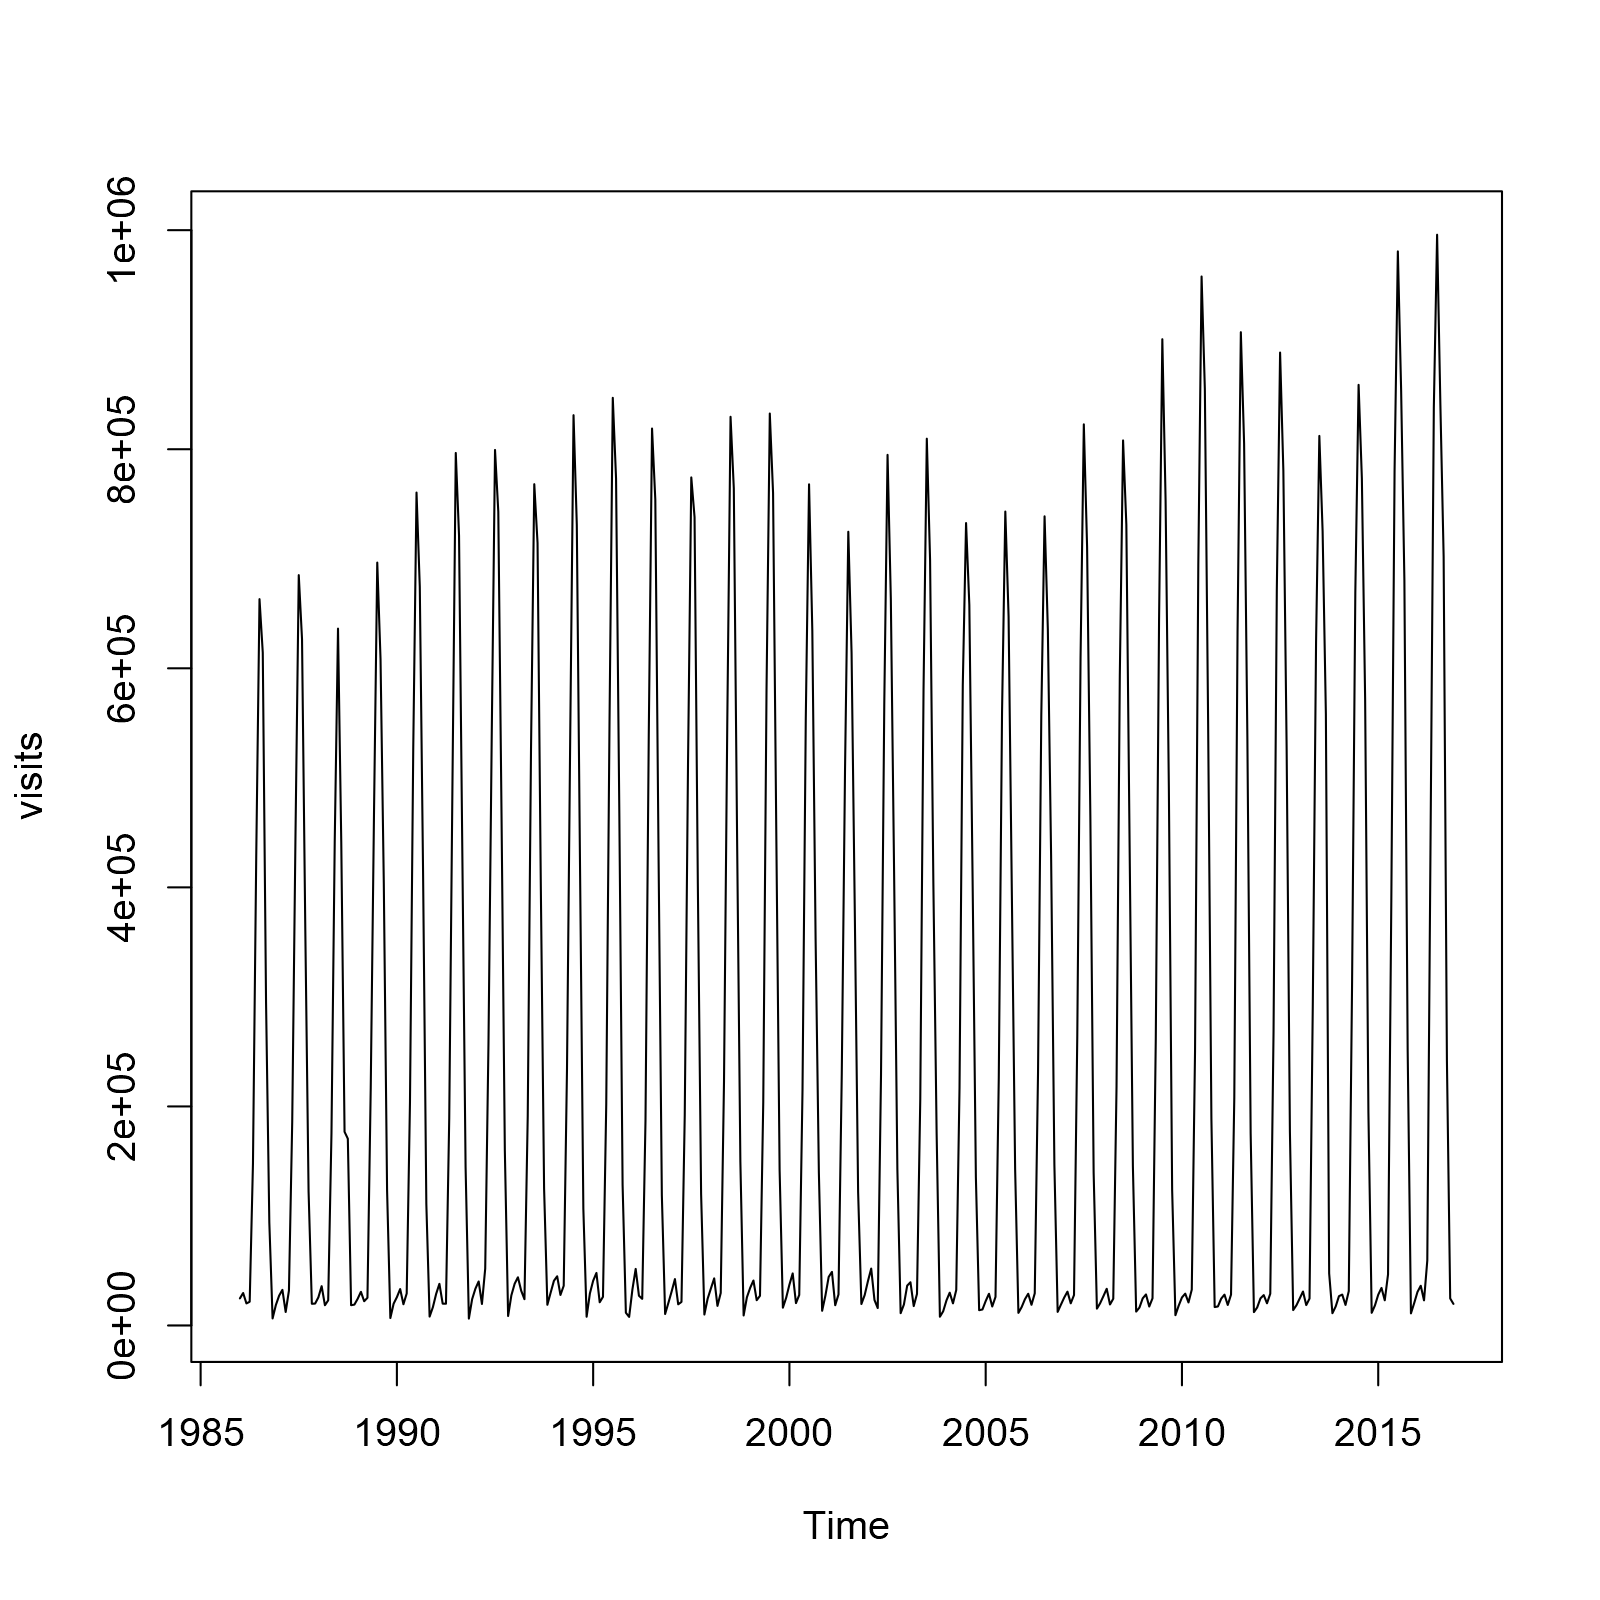
\includegraphics[width=.63\linewidth]{../normalplots/visits-ts-plot.png}
\end{figure}
\end{frame}


\begin{frame}{General trends of the time series}
\begin{figure}
\centering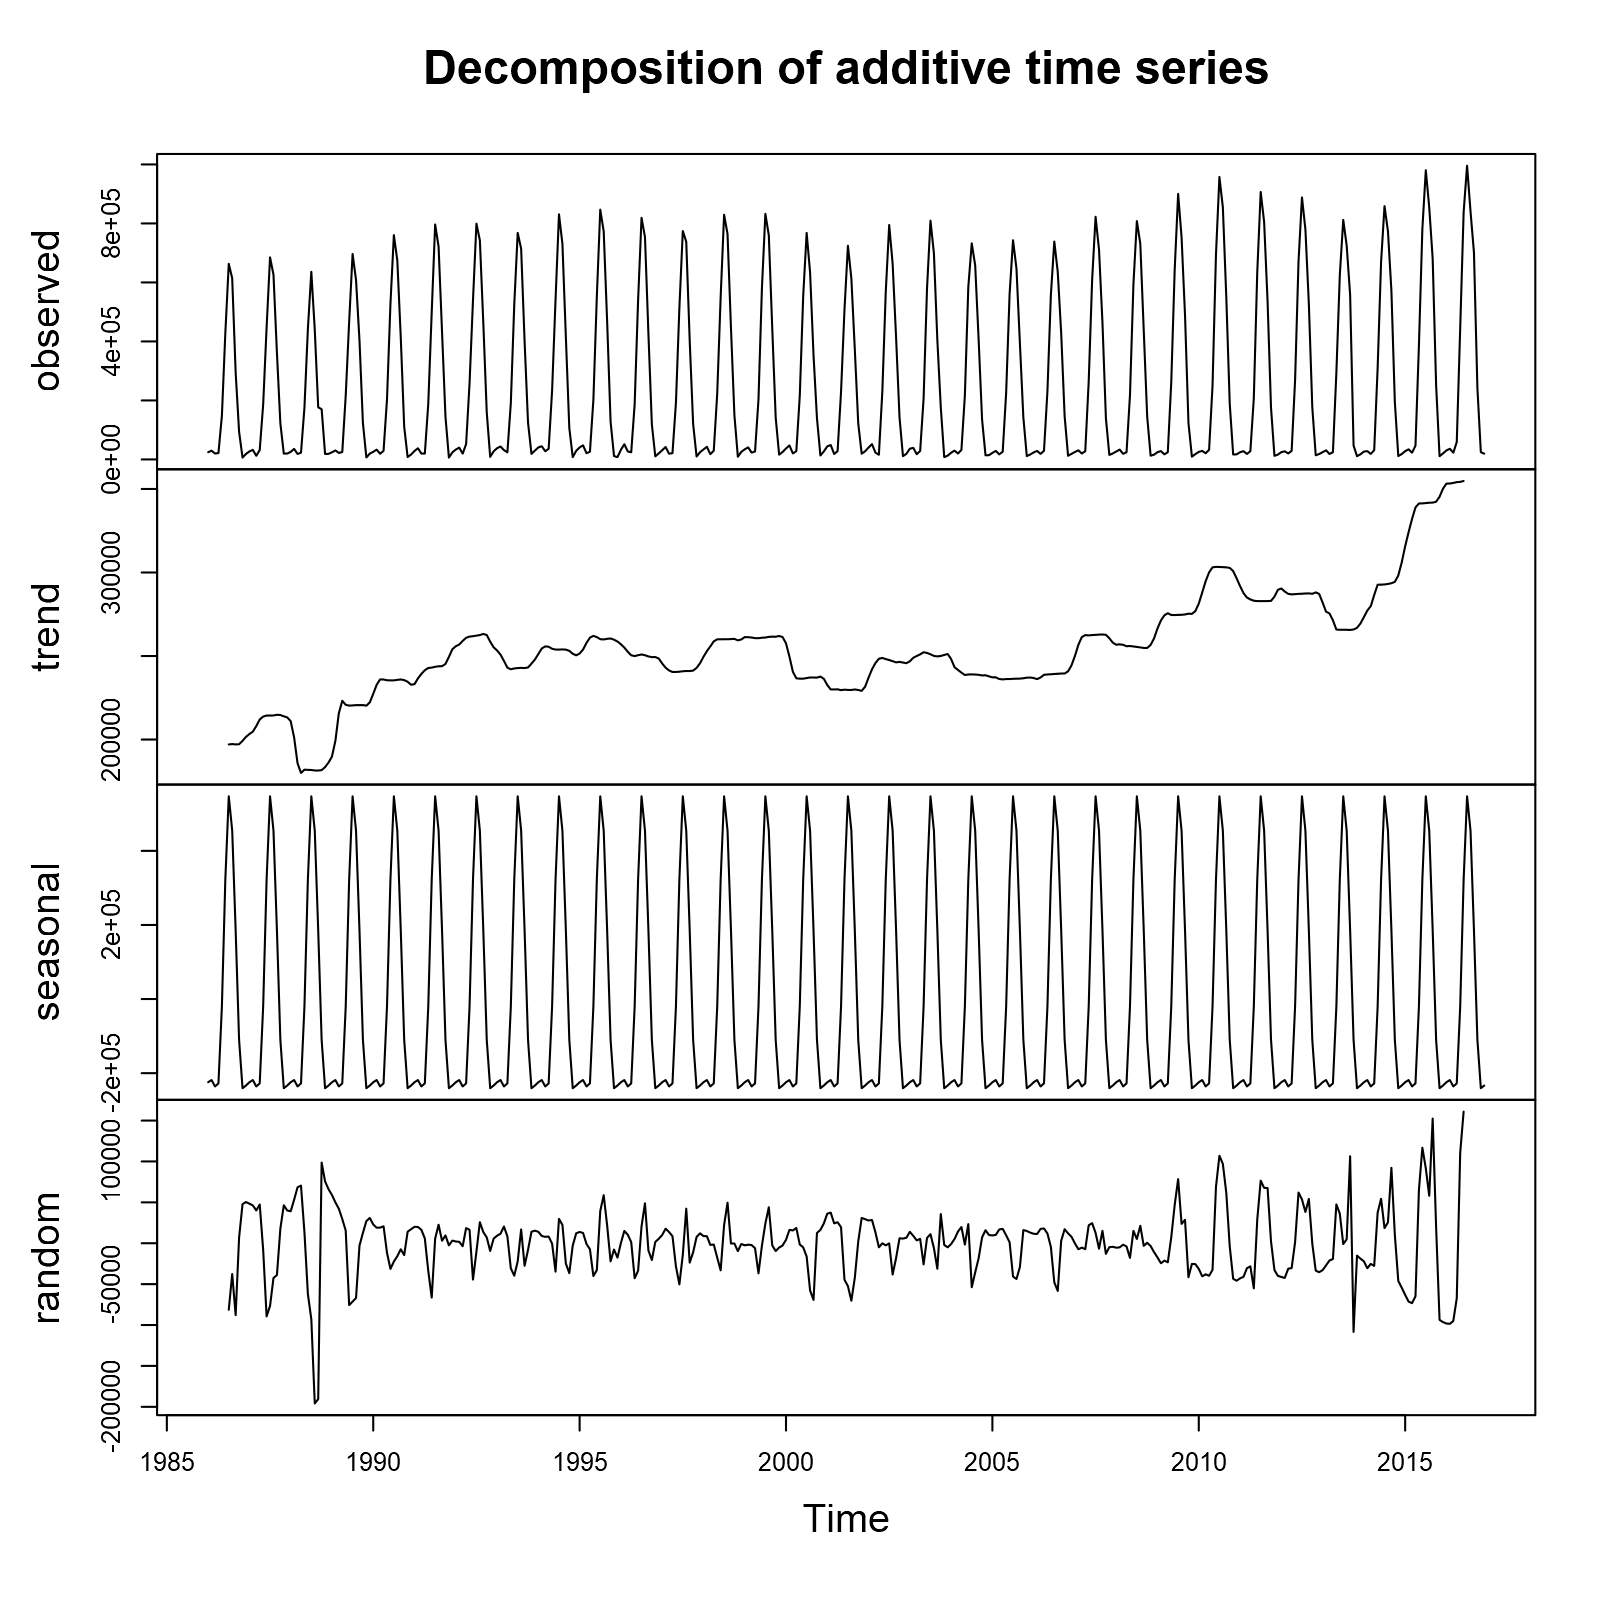
\includegraphics[width=.57\linewidth]{../normalplots/visits-components-ts-plot.png}
\end{figure}

\vfill 
\footnotesize Note the linear trend, heavy seasonality, and 1988 outlier

\end{frame}

\begin{frame}{Log transform to reduce linear trend}
\begin{figure}
\centering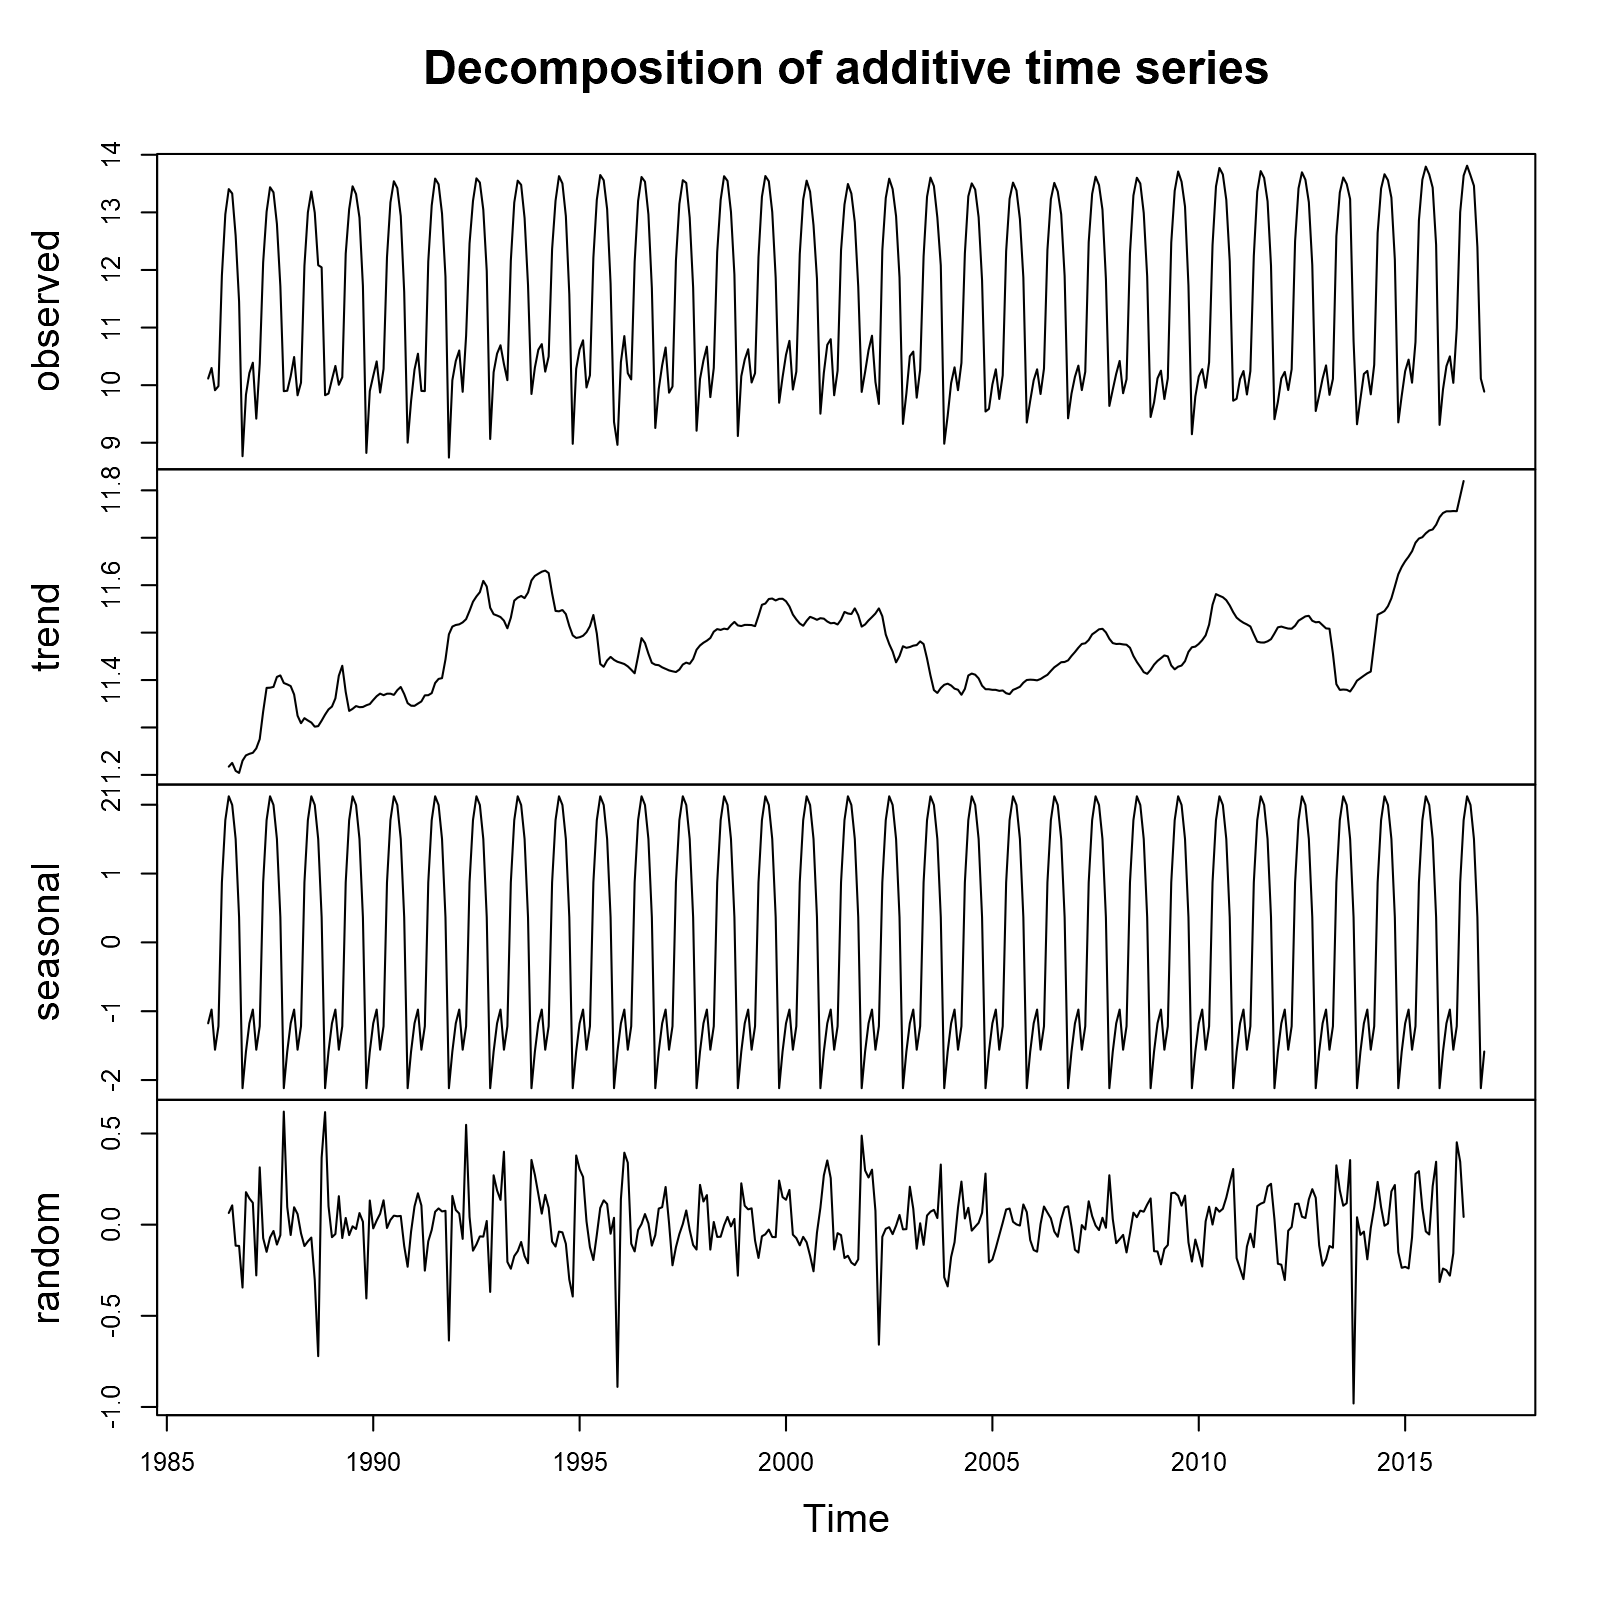
\includegraphics[width=.57\linewidth]{../normalplots/Logvisits-ts-plot.png}
\end{figure}

\vfill 
\footnotesize With the transform the trend is decreased, but we have more peaks in our random error
\end{frame}


\begin{frame}{Seasonality}

\small{\textbf{Distribution without transformation}\hfill \textbf{Distribution with log transformation}}
\vspace{-1em}
\begin{figure}
\centering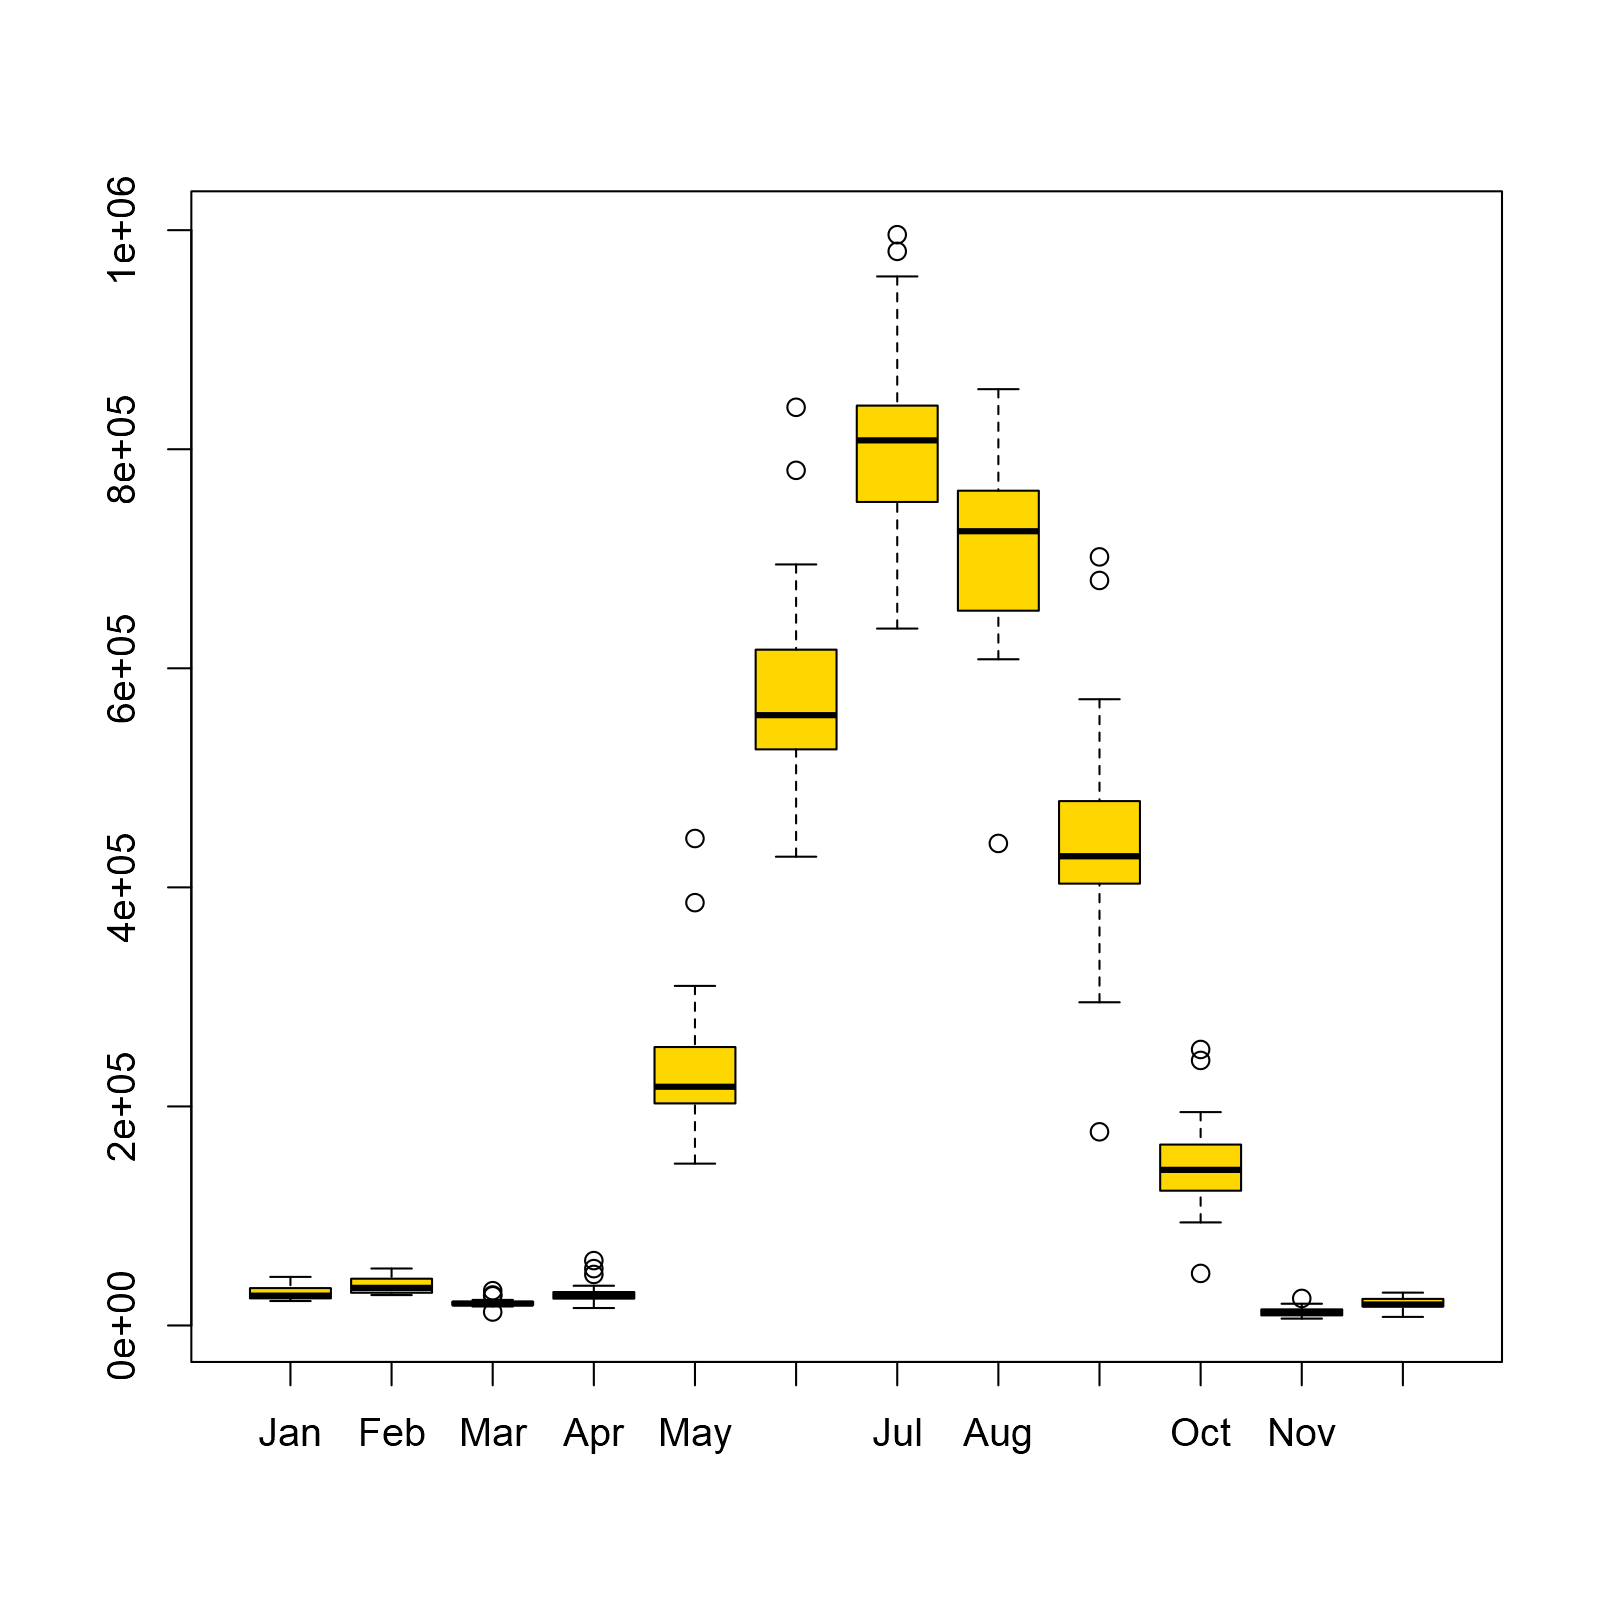
\includegraphics[width=.47\linewidth]{../normalplots/visits-distribution-plot.png} \hfill \centering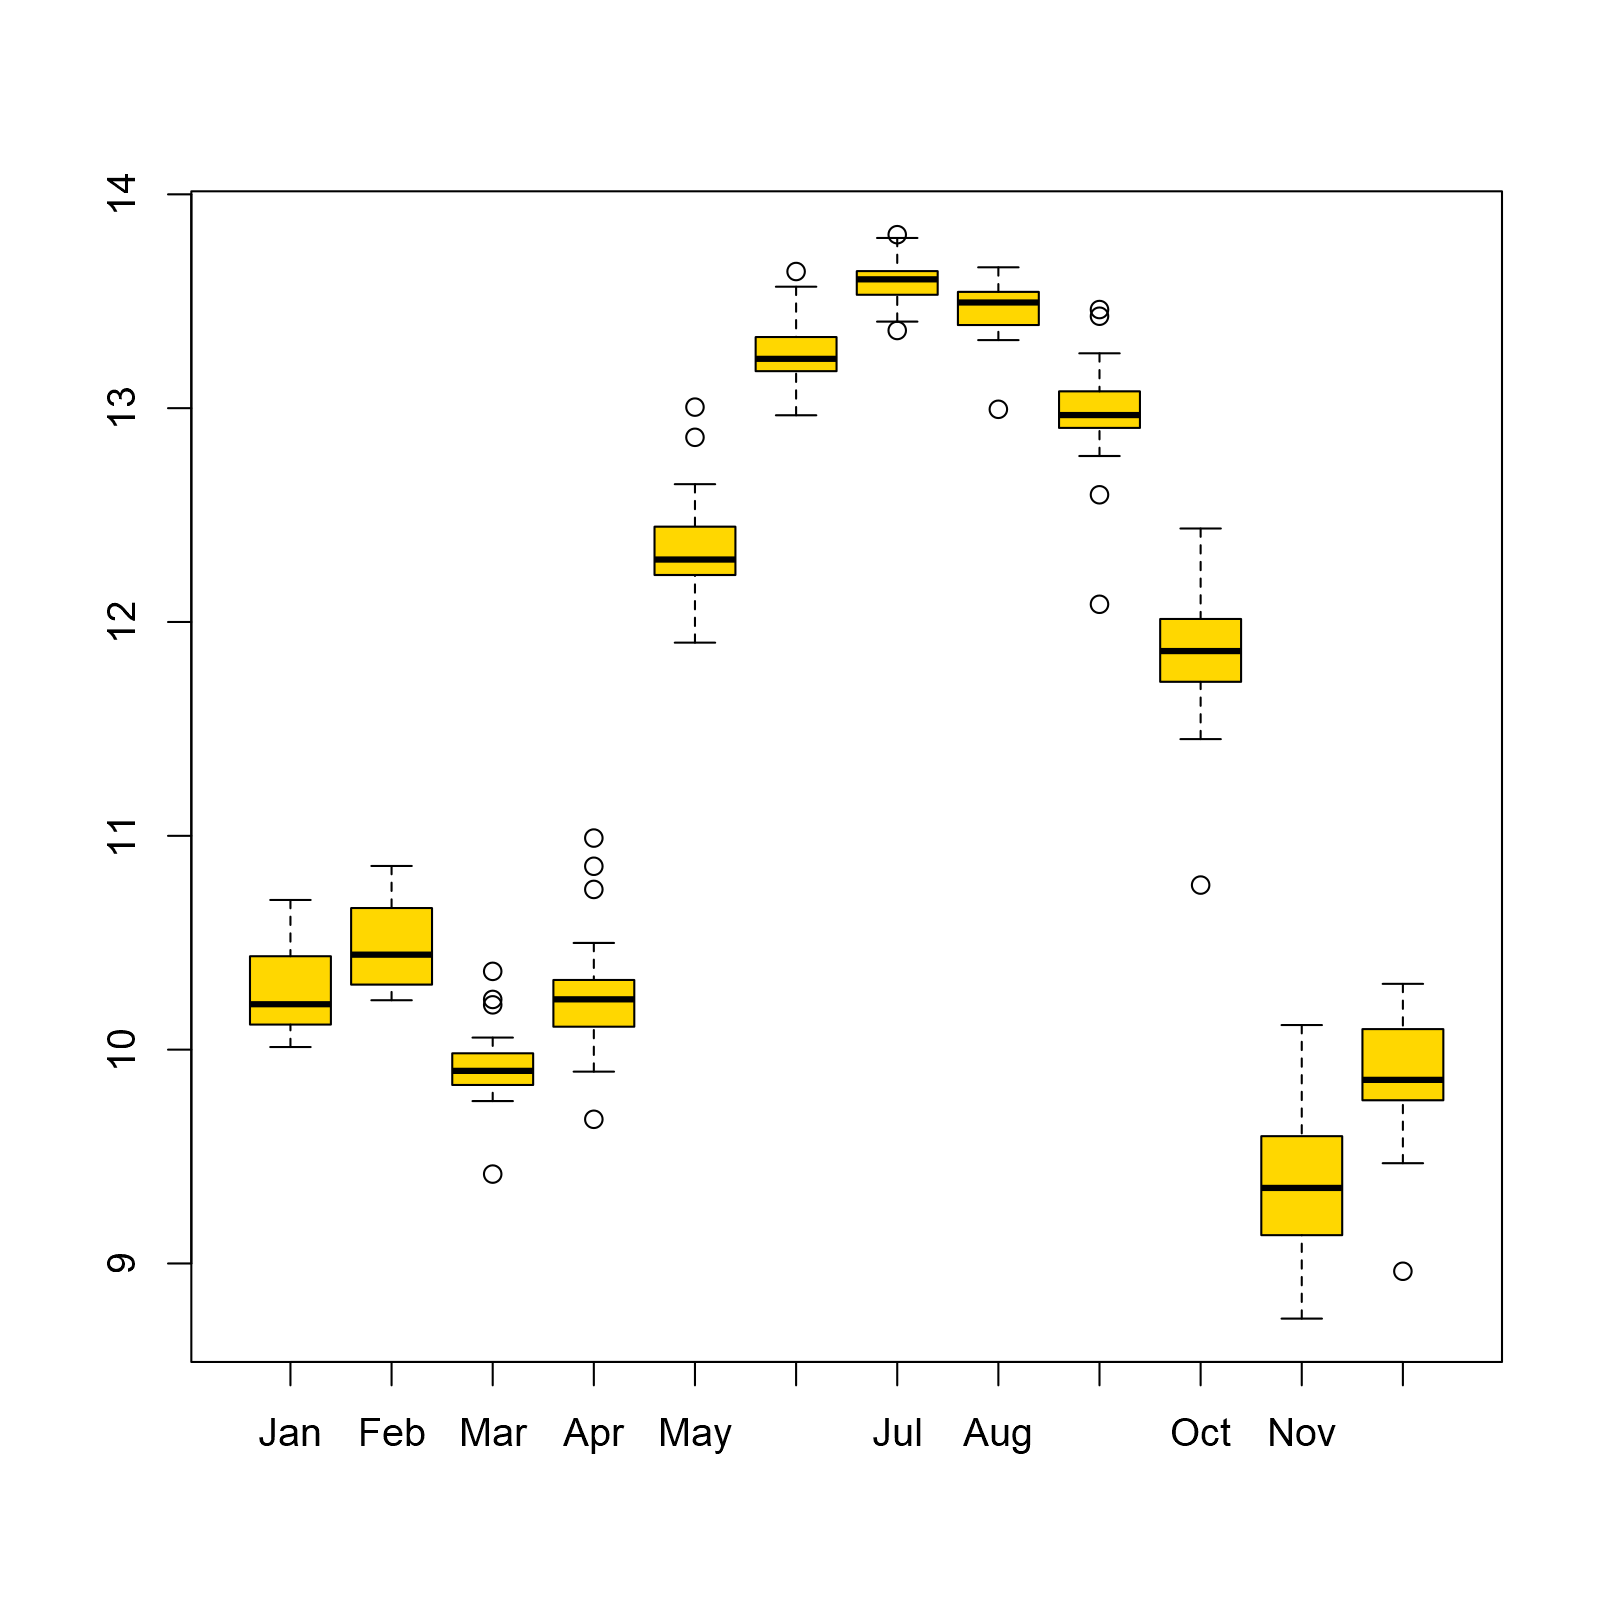
\includegraphics[width=.47\linewidth]{../normalplots/logvisits-distribution-plot.png}
\end{figure}

\vfill 
\footnotesize Summer months have drastic increase in visitors


\end{frame}

\section{Model Fitting}
\subsection{}

\begin{frame}{Model Choice}
\begin{itemize}
\item Both series had p values of less than .01 with Augmented Dickey-Fuller Test
\item Held last year of data from each series in order to check the accuracy of our forecasts
\item Systematically chose models with the lowest AIC value for our two series to get the following
\item \textbf{Regular data: } AR(1) model with a seasonal component of order (0,1,1) 
\item \textbf{Log transform:} MA(1) model with a seasonal component of  order (2,1,1)

\end{itemize}
\end{frame}


\begin{frame}{Model Diagnostics: ARIMA (1,0,0) X (0,1,1) [data without transformation]}
\begin{figure}
\centering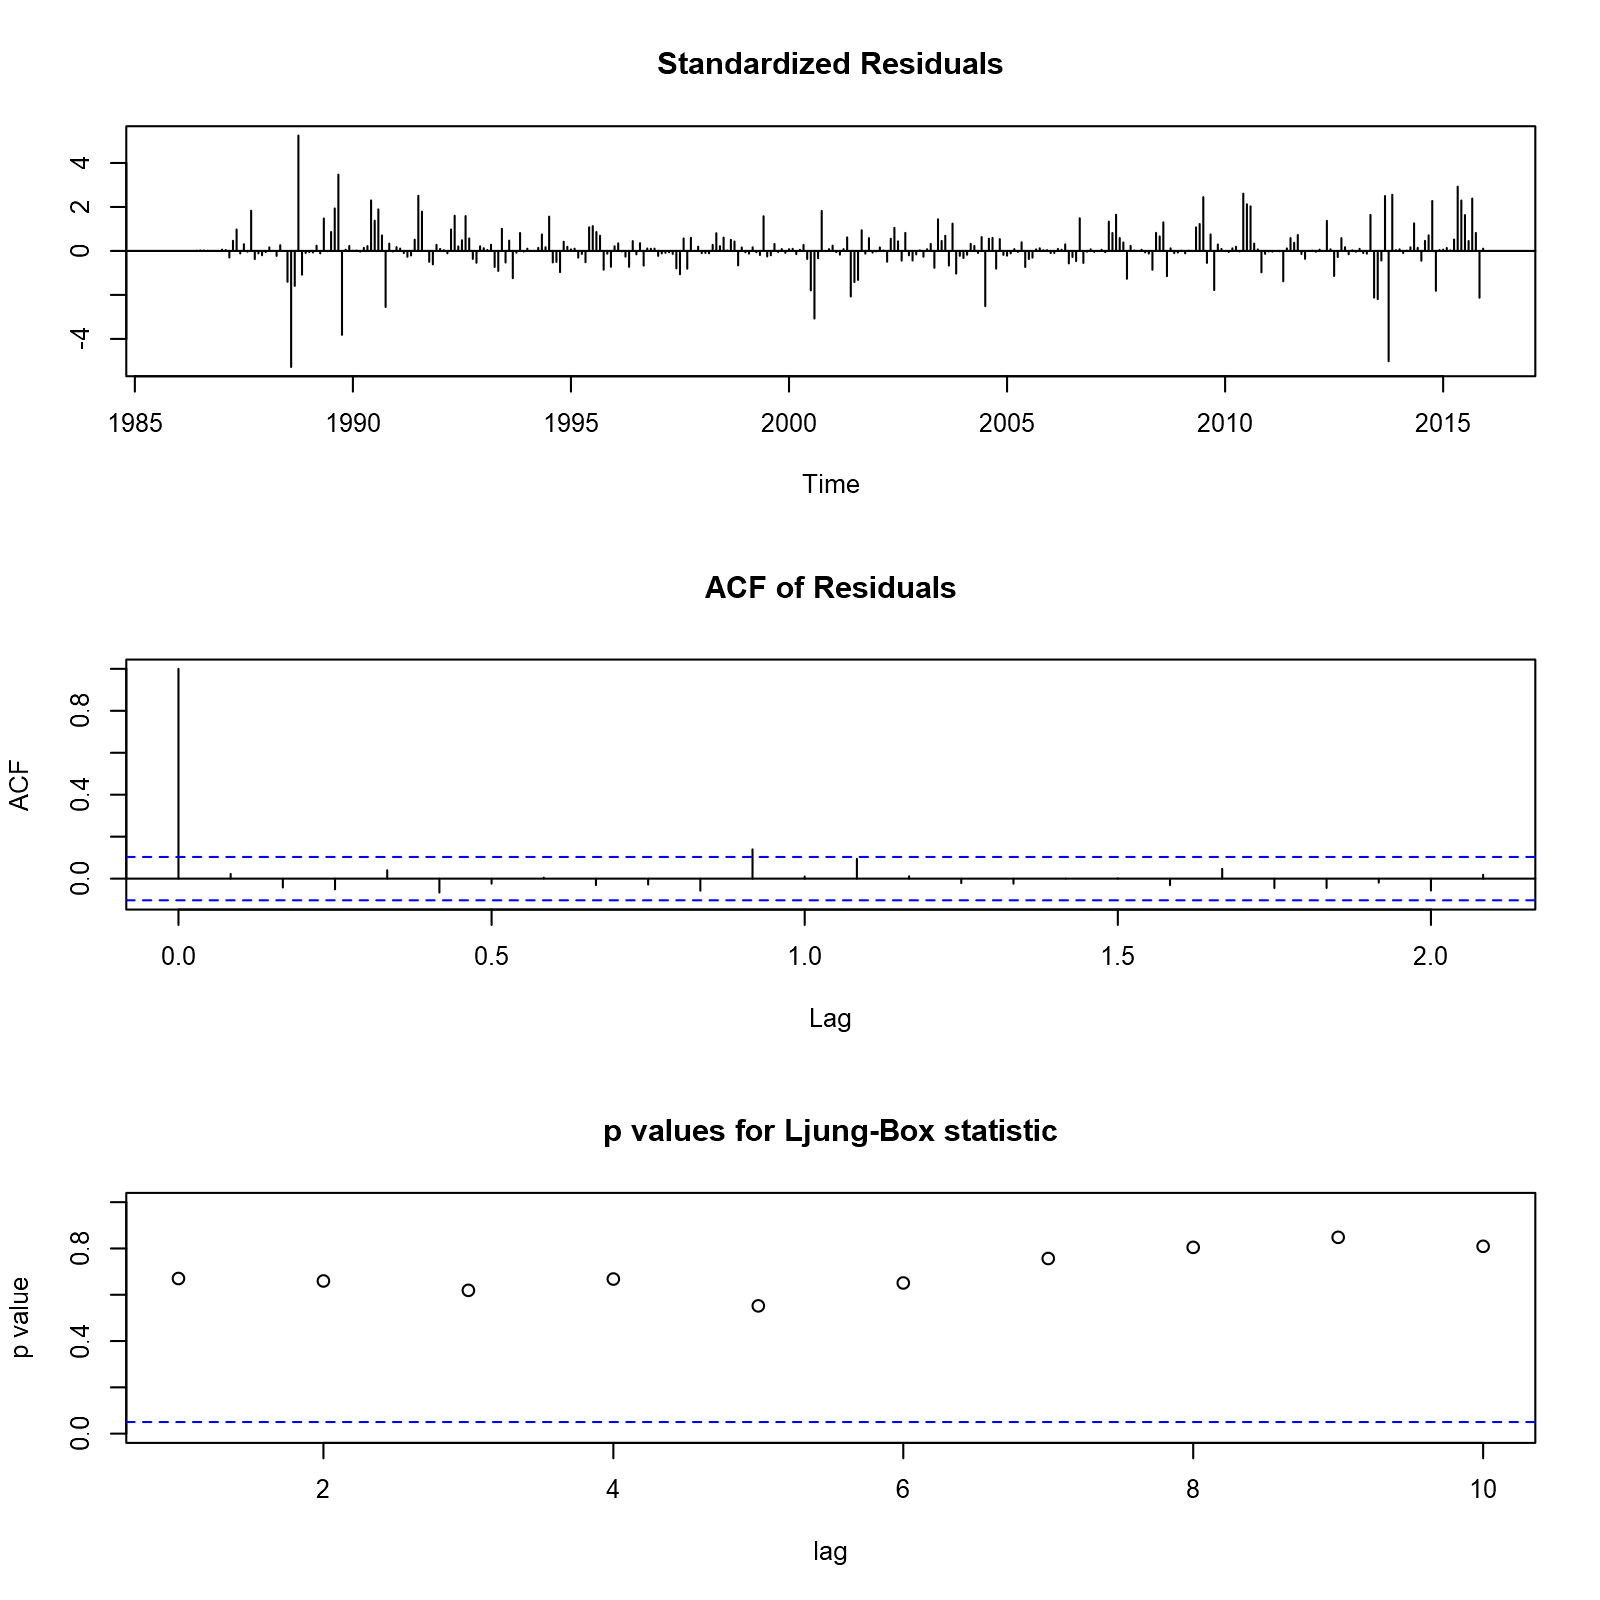
\includegraphics[width=.48\linewidth]{../normalplots/tsdiag-fitV-plot.png}
\end{figure}

\vfill 
\footnotesize Again note the 1988 outlier and that the Ljung-Box statistic is significant up to a lag of 15 

\end{frame}


\begin{frame}{Model Diagnostics: ARIMA (0,0,1) X (2,1,1) [data with transformation]}
\begin{figure}
\centering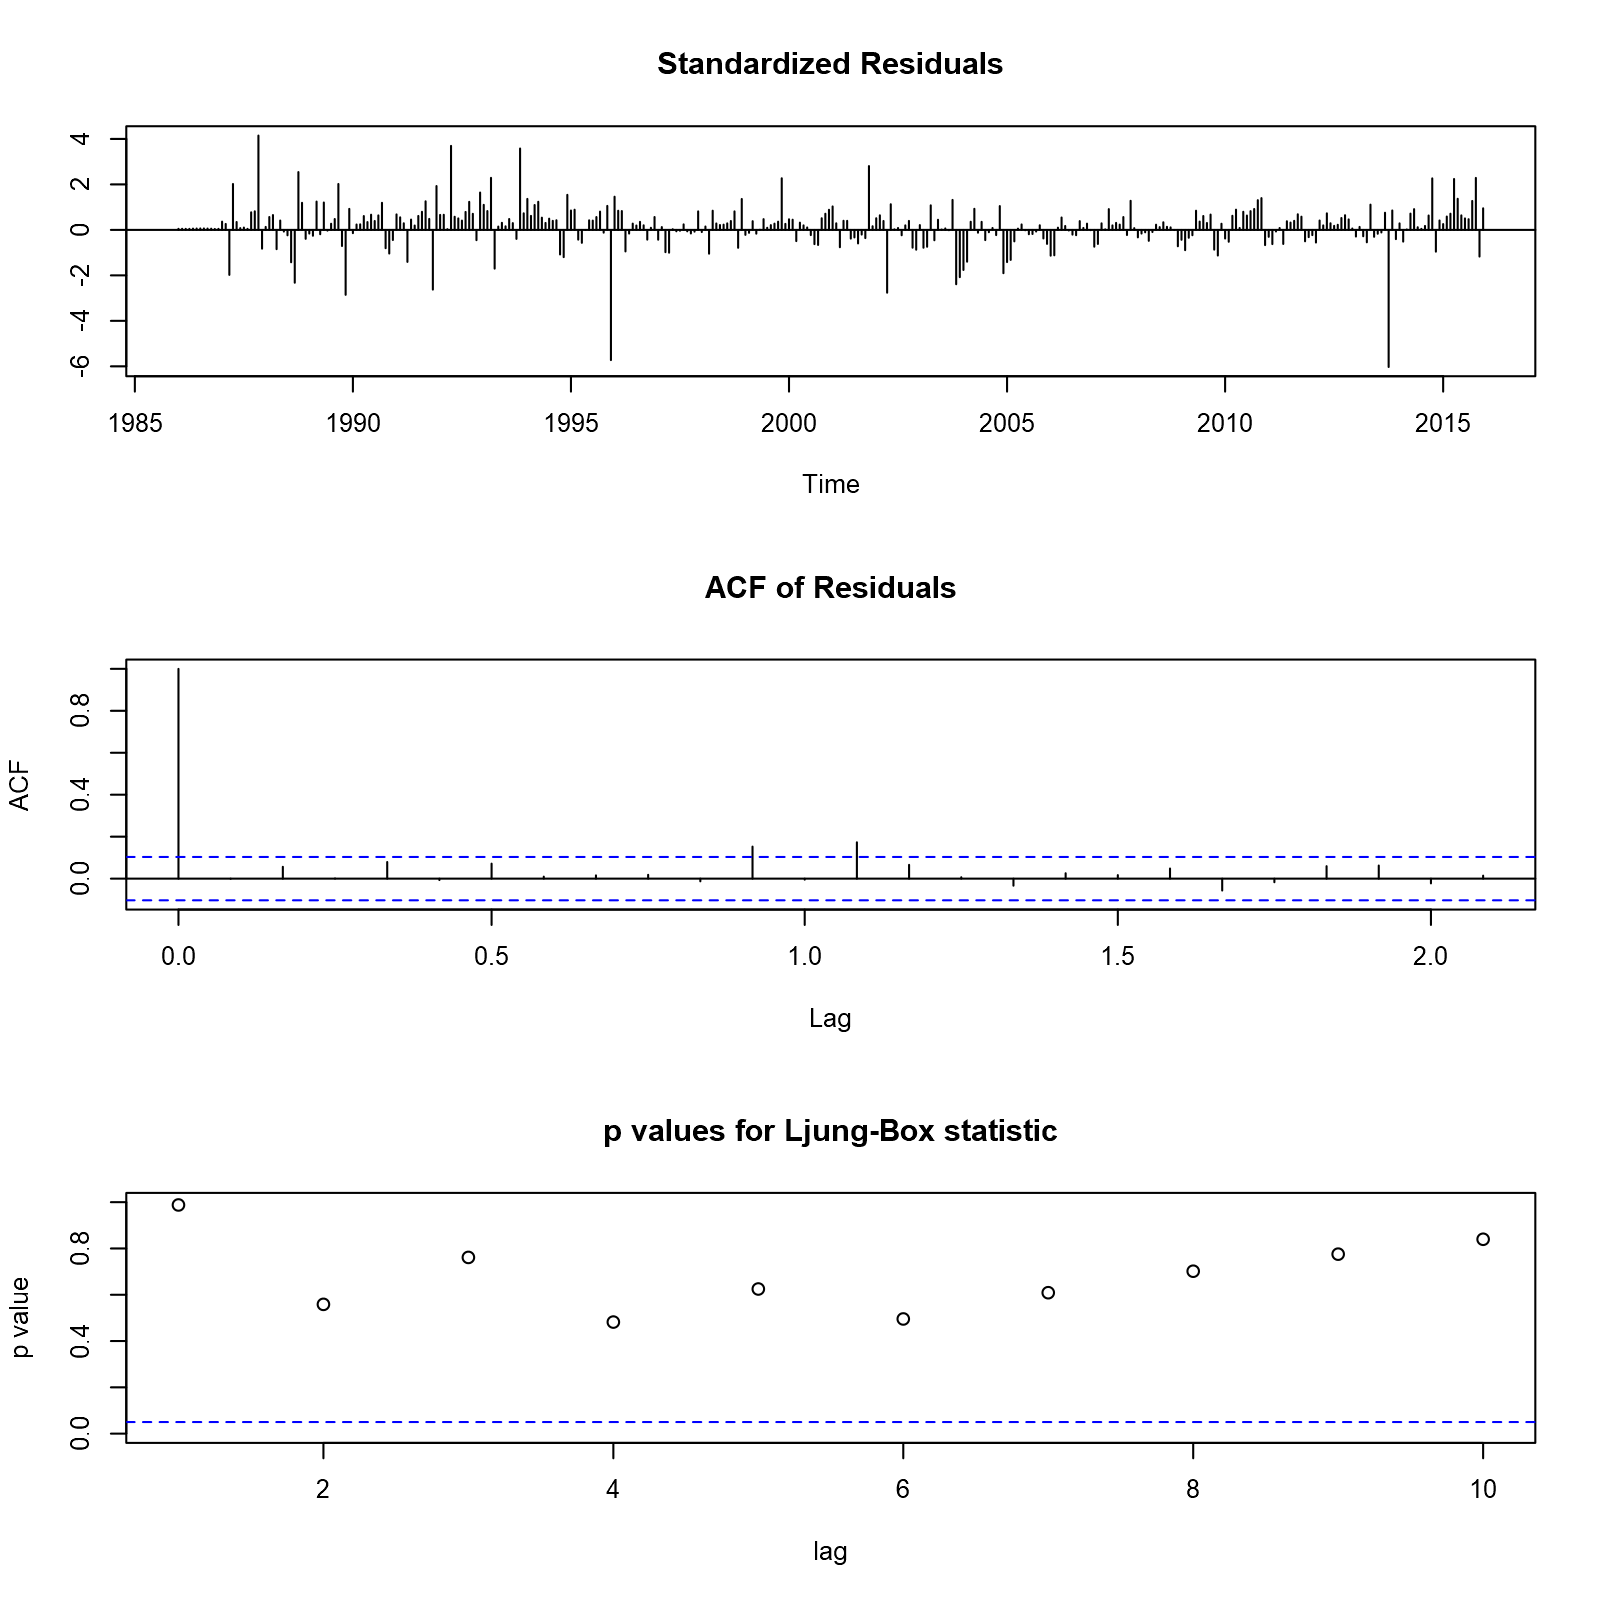
\includegraphics[width=.45\linewidth]{../normalplots/tsdiag-fitLV-plot.png}
\end{figure}

\vfill 
\footnotesize With the transform the trend is decreased, but we have more peaks in our random error. Also the Ljung-Box statistic for the transformed data is only significant up to a lag of 12 
\end{frame}

\section{Forecasting}
\subsection{}

\begin{frame}{Forecast of model without log transformation}

\vspace{-1em}
\begin{figure}
\centering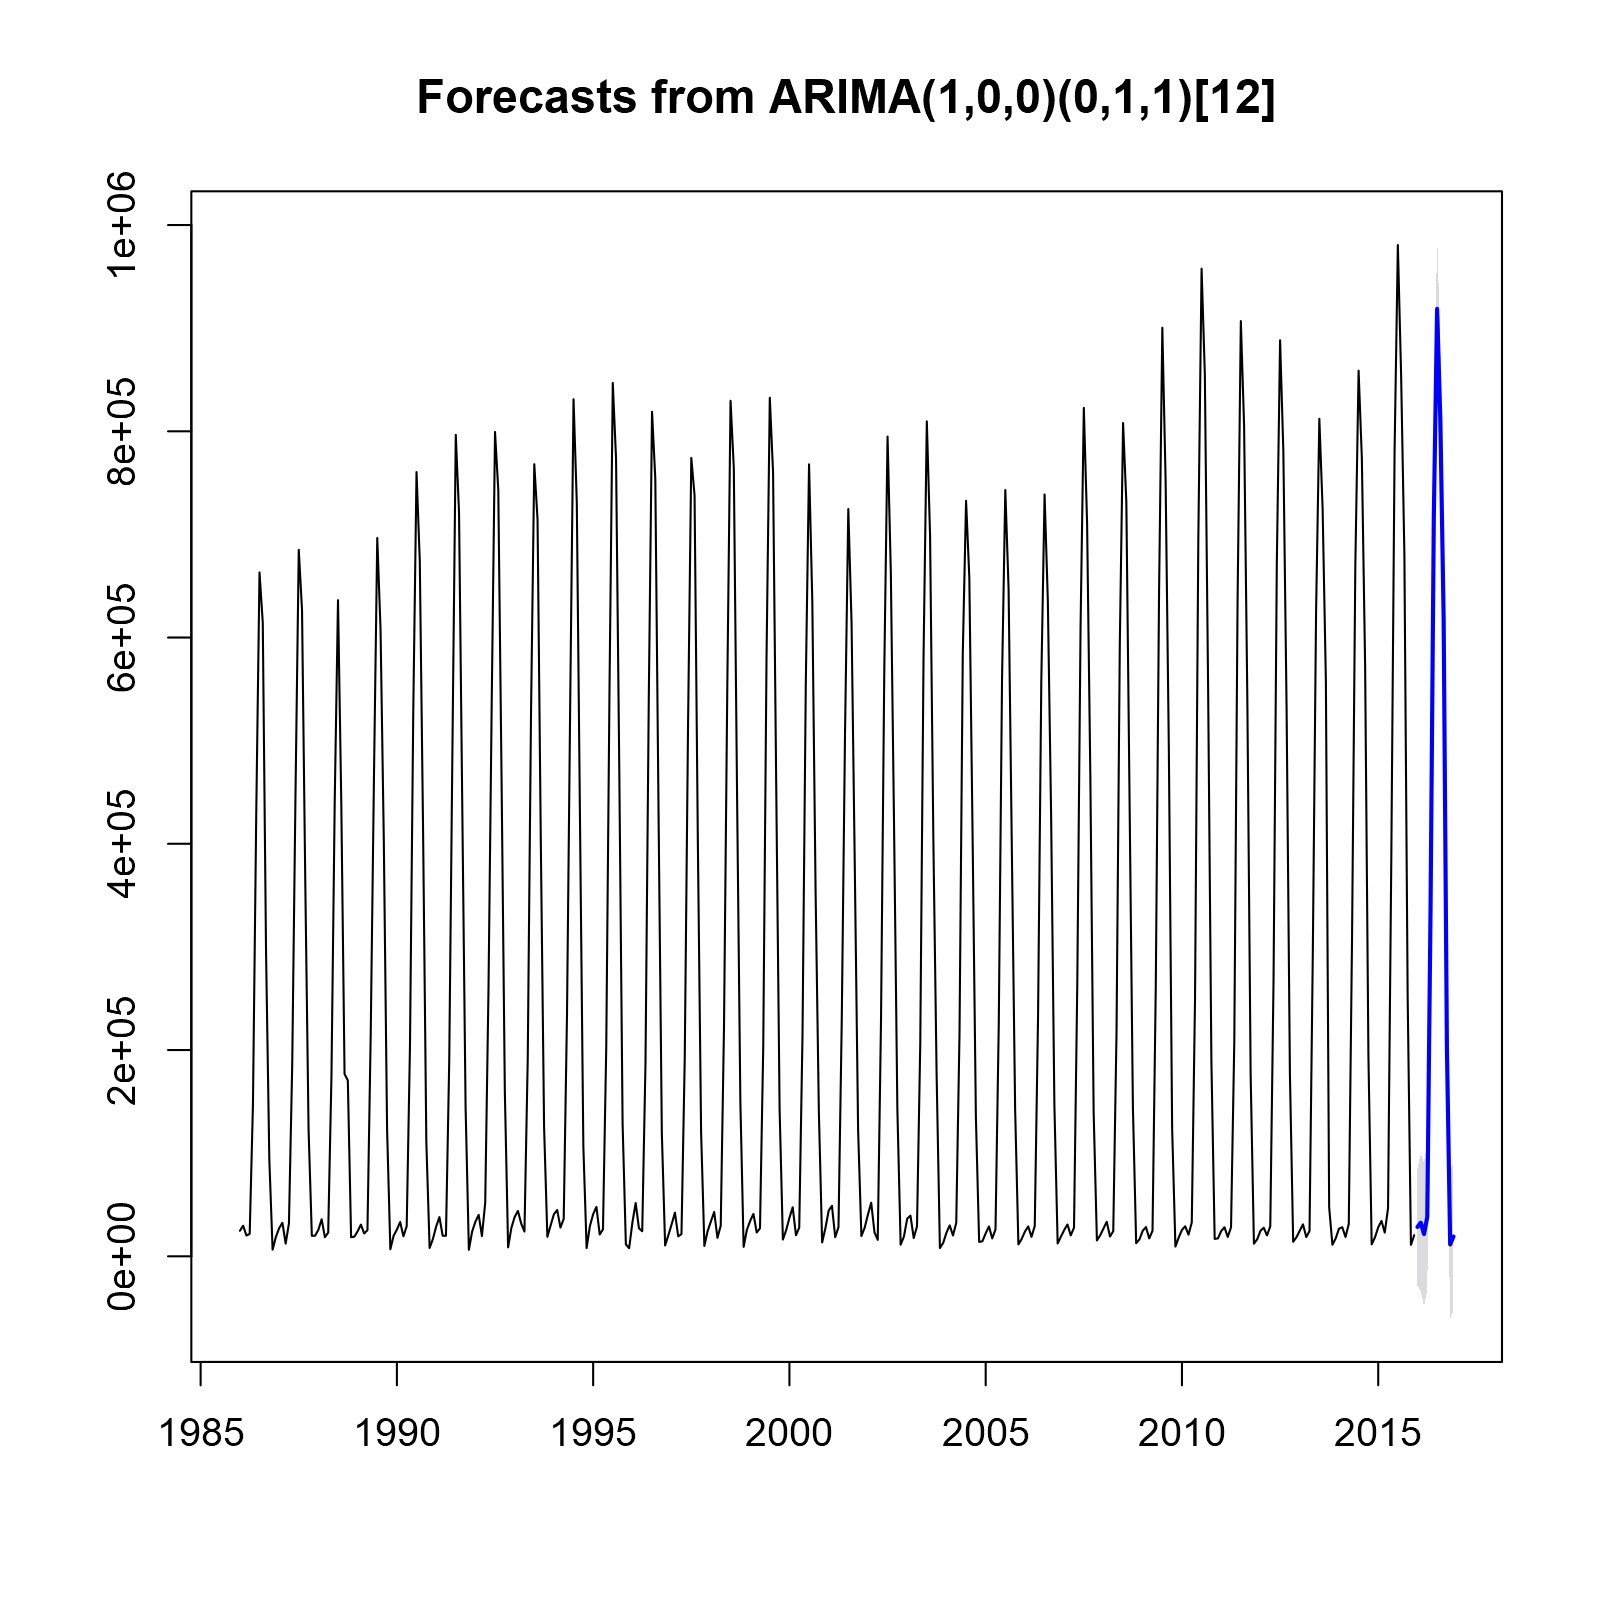
\includegraphics[width=.47\linewidth]{../normalplots/forecast95-fitV-plot.png} \hfill \centering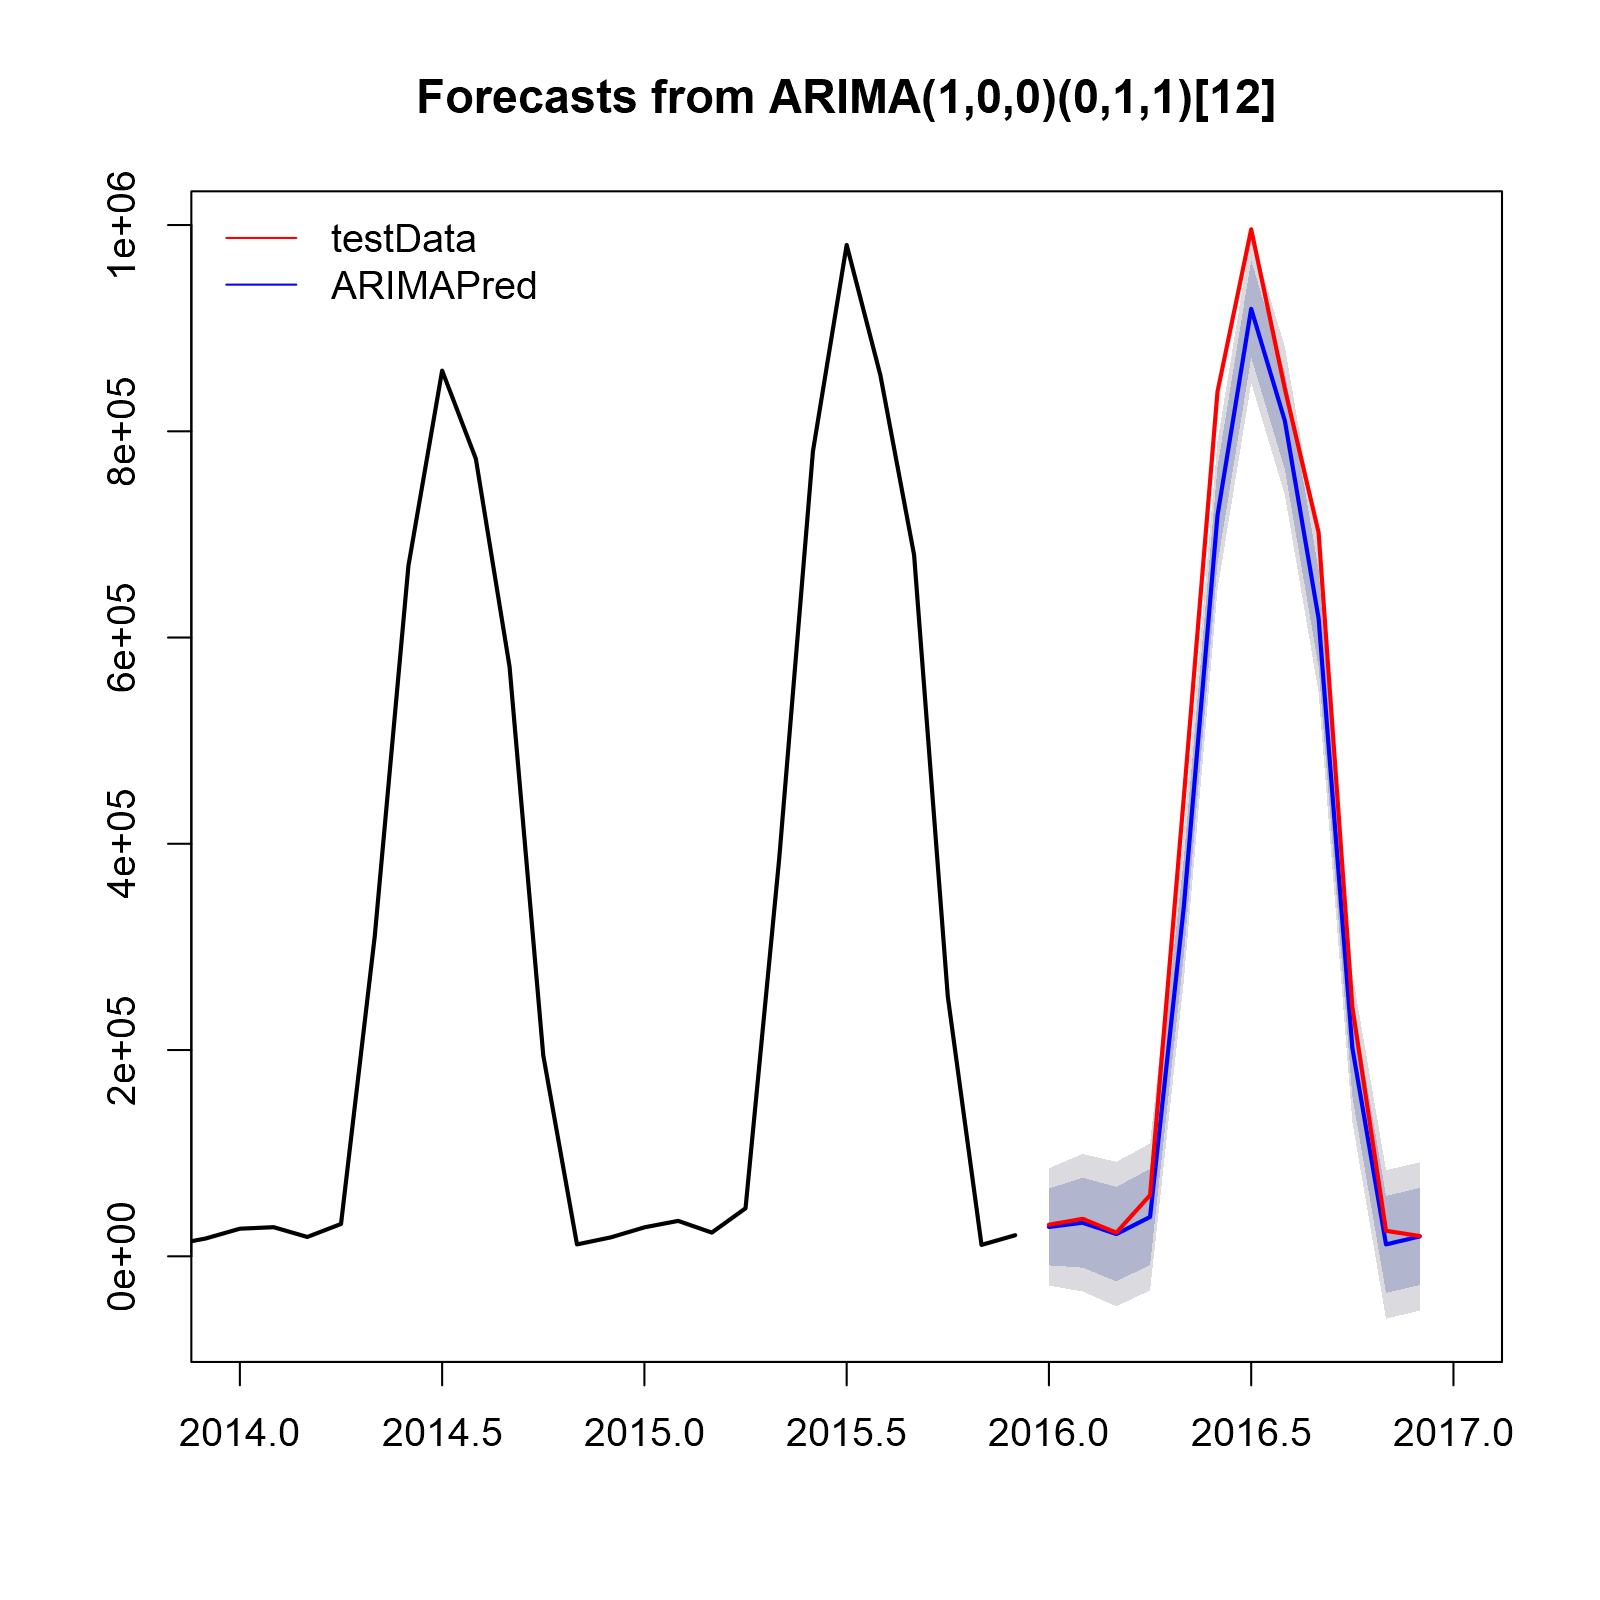
\includegraphics[width=.47\linewidth]{../normalplots/forecastGOOD-fitV-plot.png}
\end{figure}

\vfill 
%\footnotesize non log forecast comment
\end{frame}

\begin{frame}{Forecast of model with log transformation}
\vspace{-1em}
\begin{figure}
\centering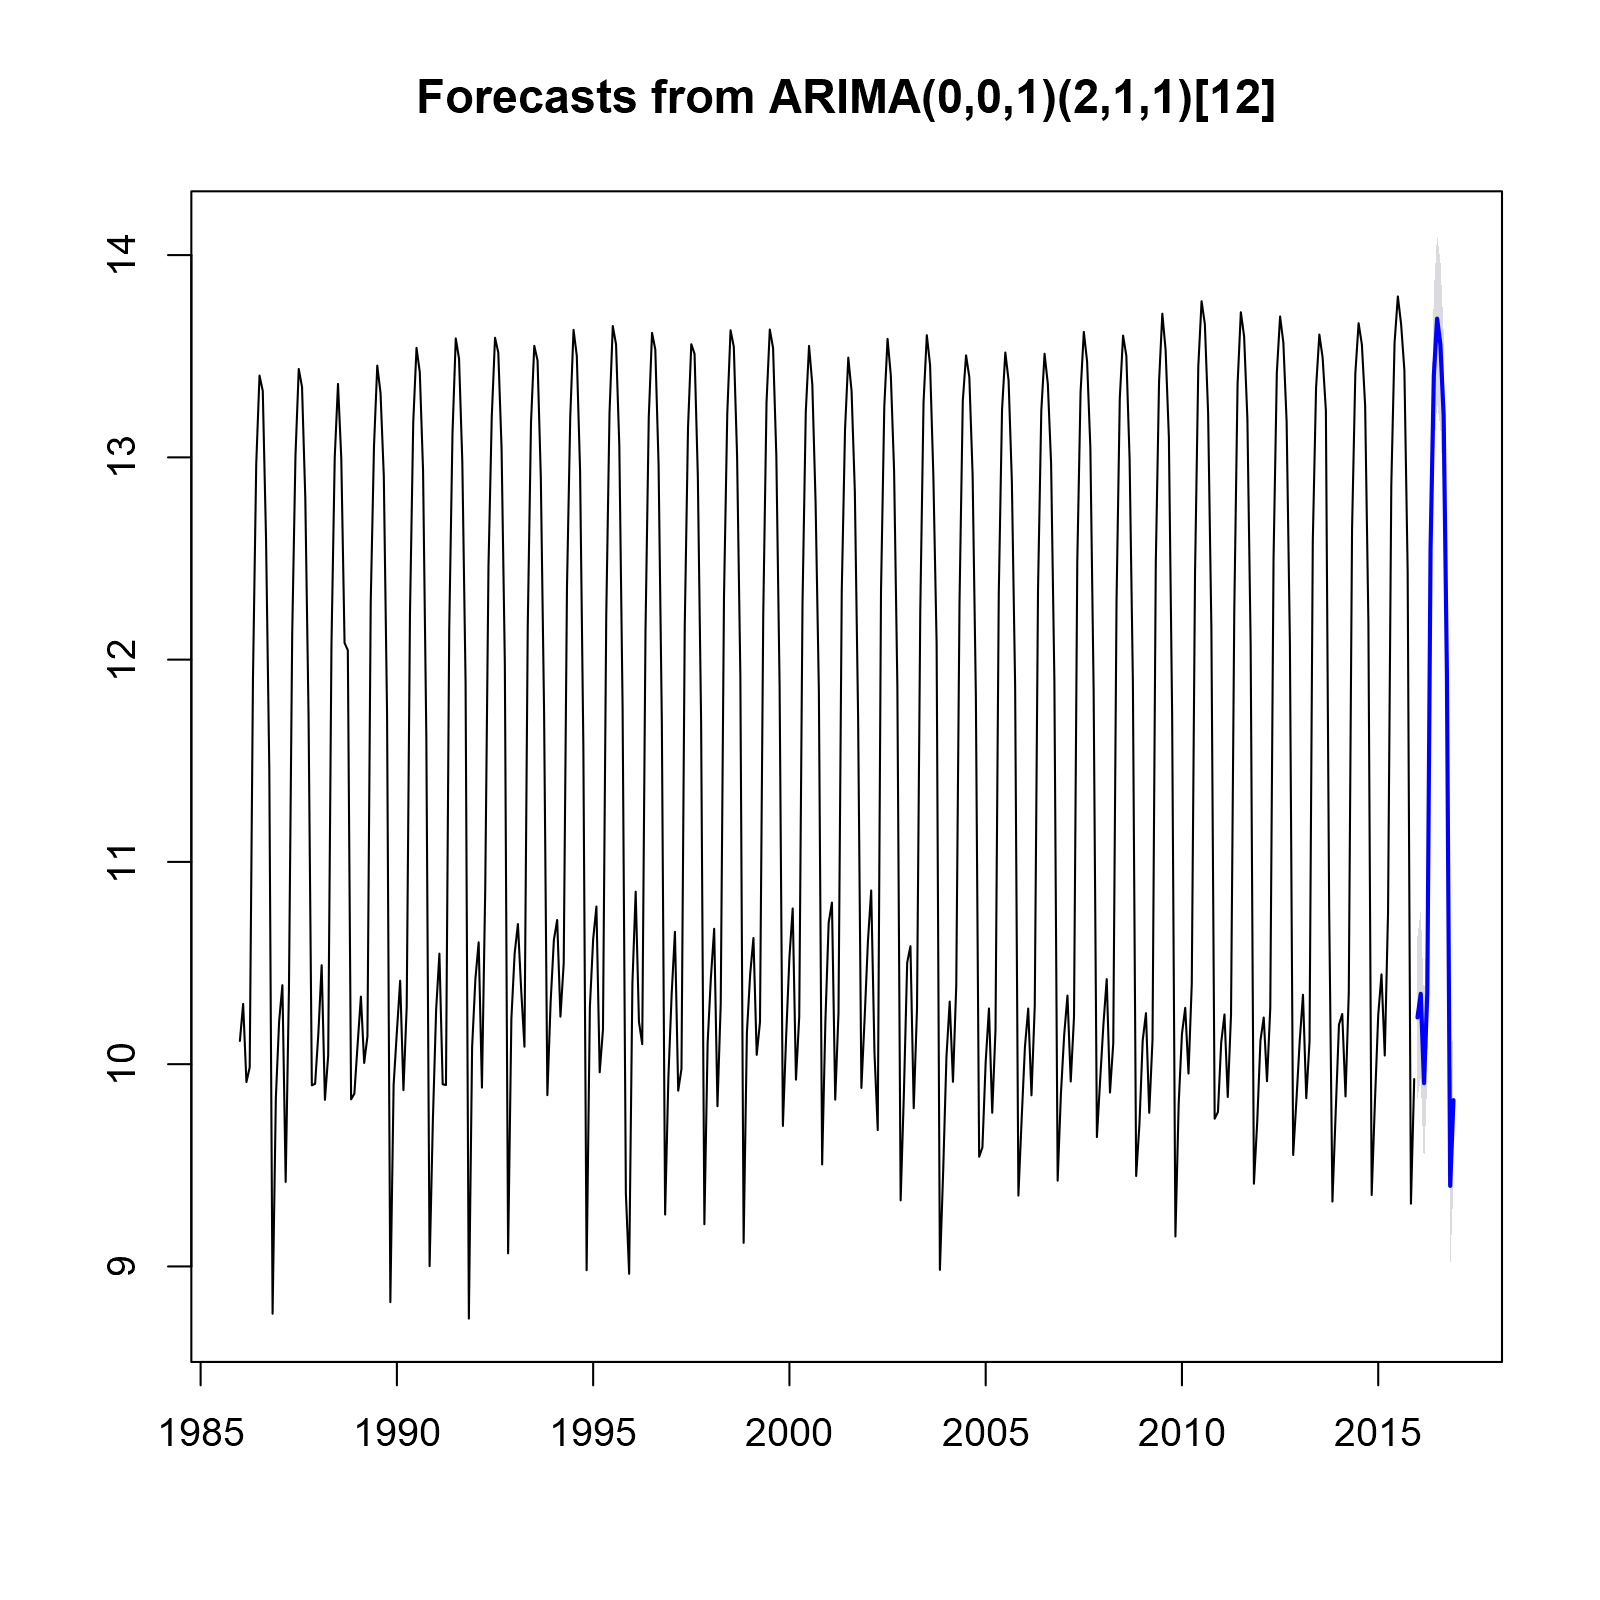
\includegraphics[width=.47\linewidth]{../normalplots/forecast95-fitLV-plot.png} \hfill \centering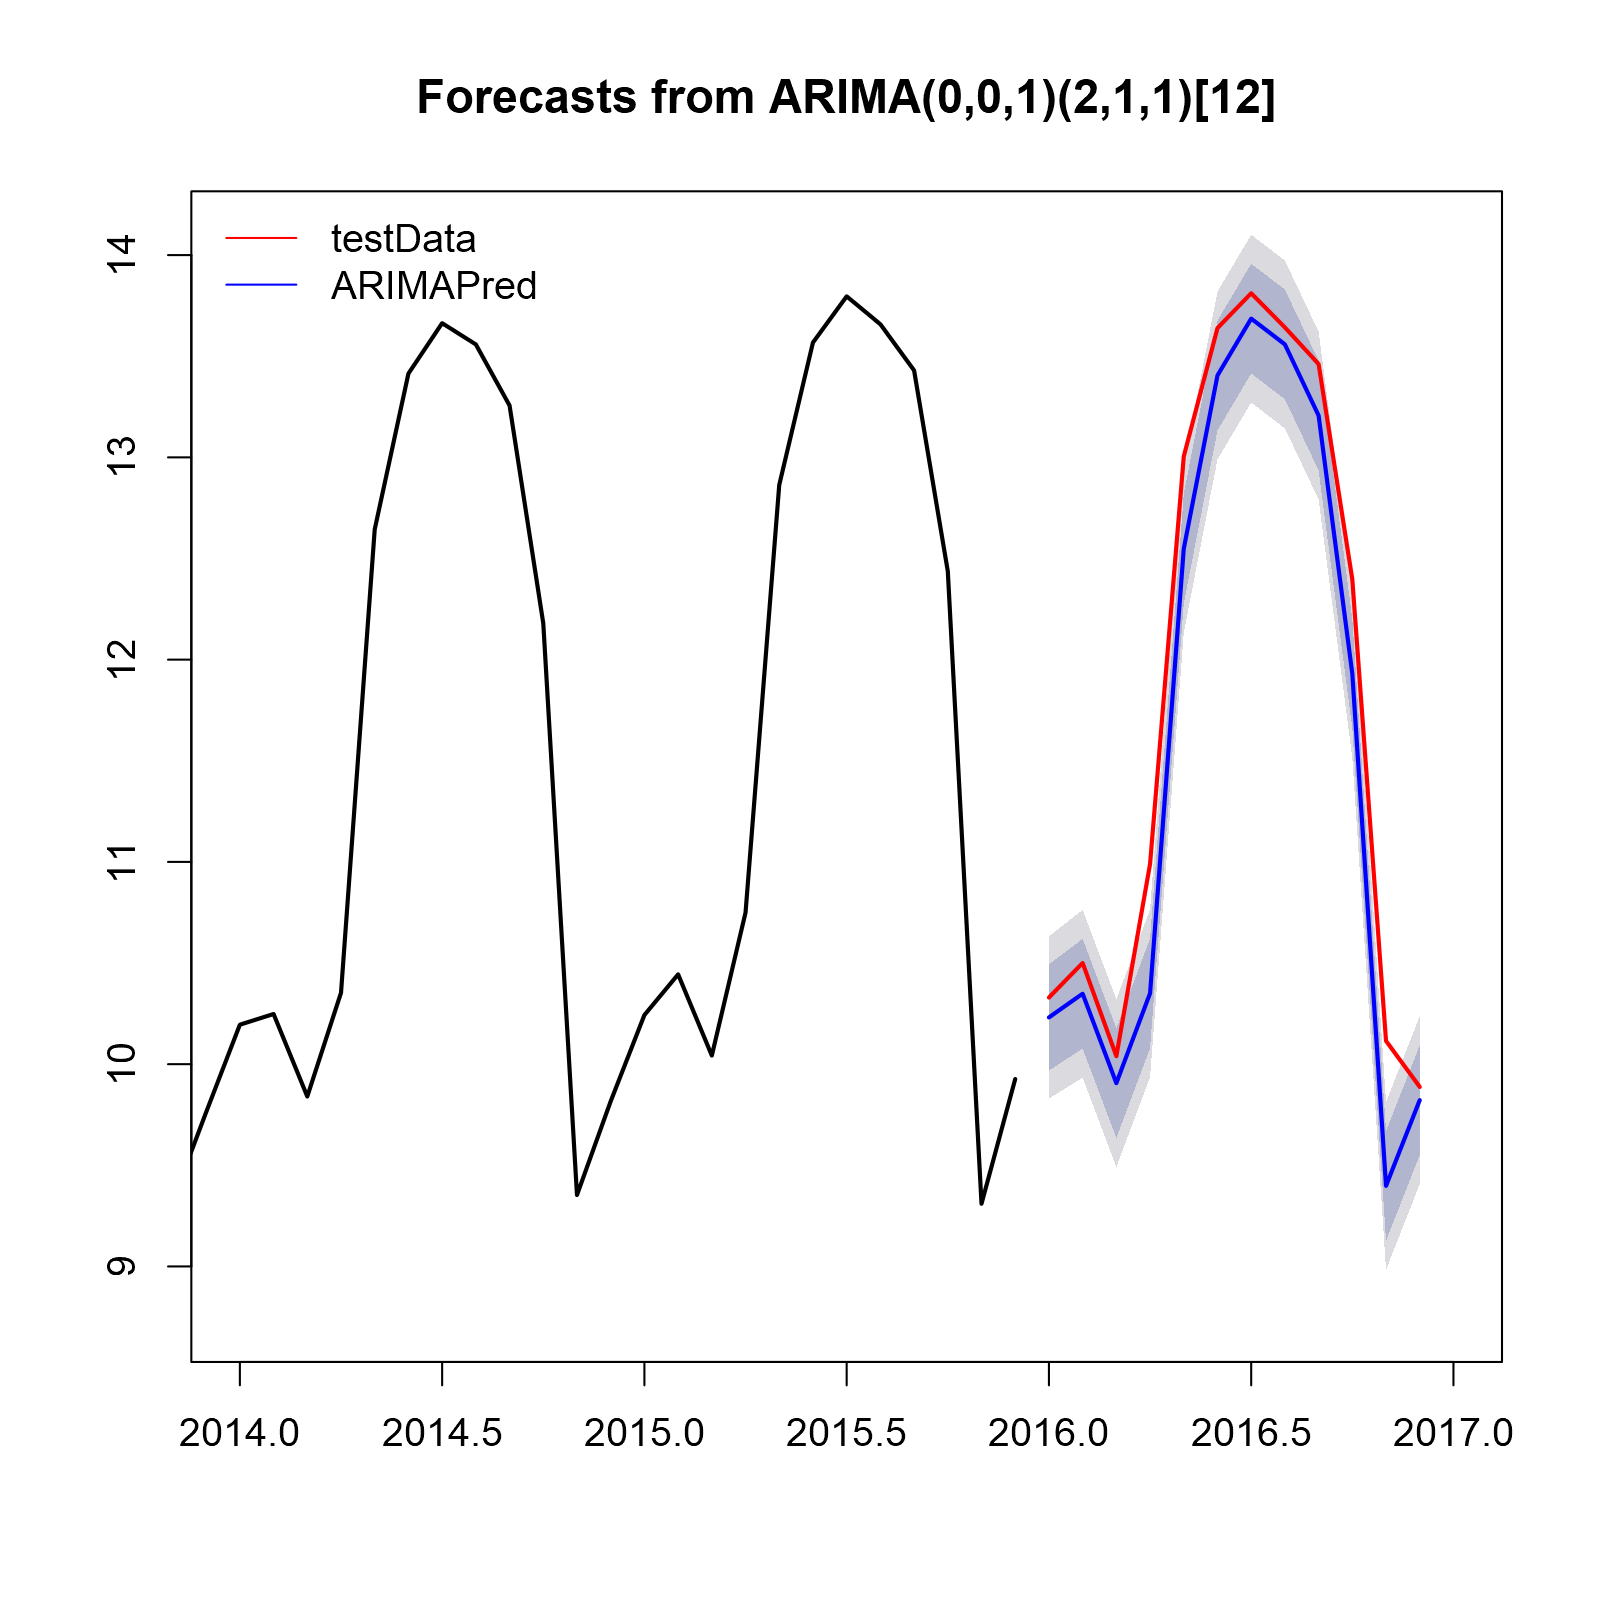
\includegraphics[width=.47\linewidth]{../normalplots/forecastGOOD-fitLV-plot.png}
\end{figure}

\vfill 
%\footnotesize log forecast comment  %
\end{frame}

\begin{frame}{Comparison of the two forecasts}
\small{\textbf{Model on regular data}\hfill \textbf{Model on log transformation}}
\vspace{-1em}
\begin{figure}
\centering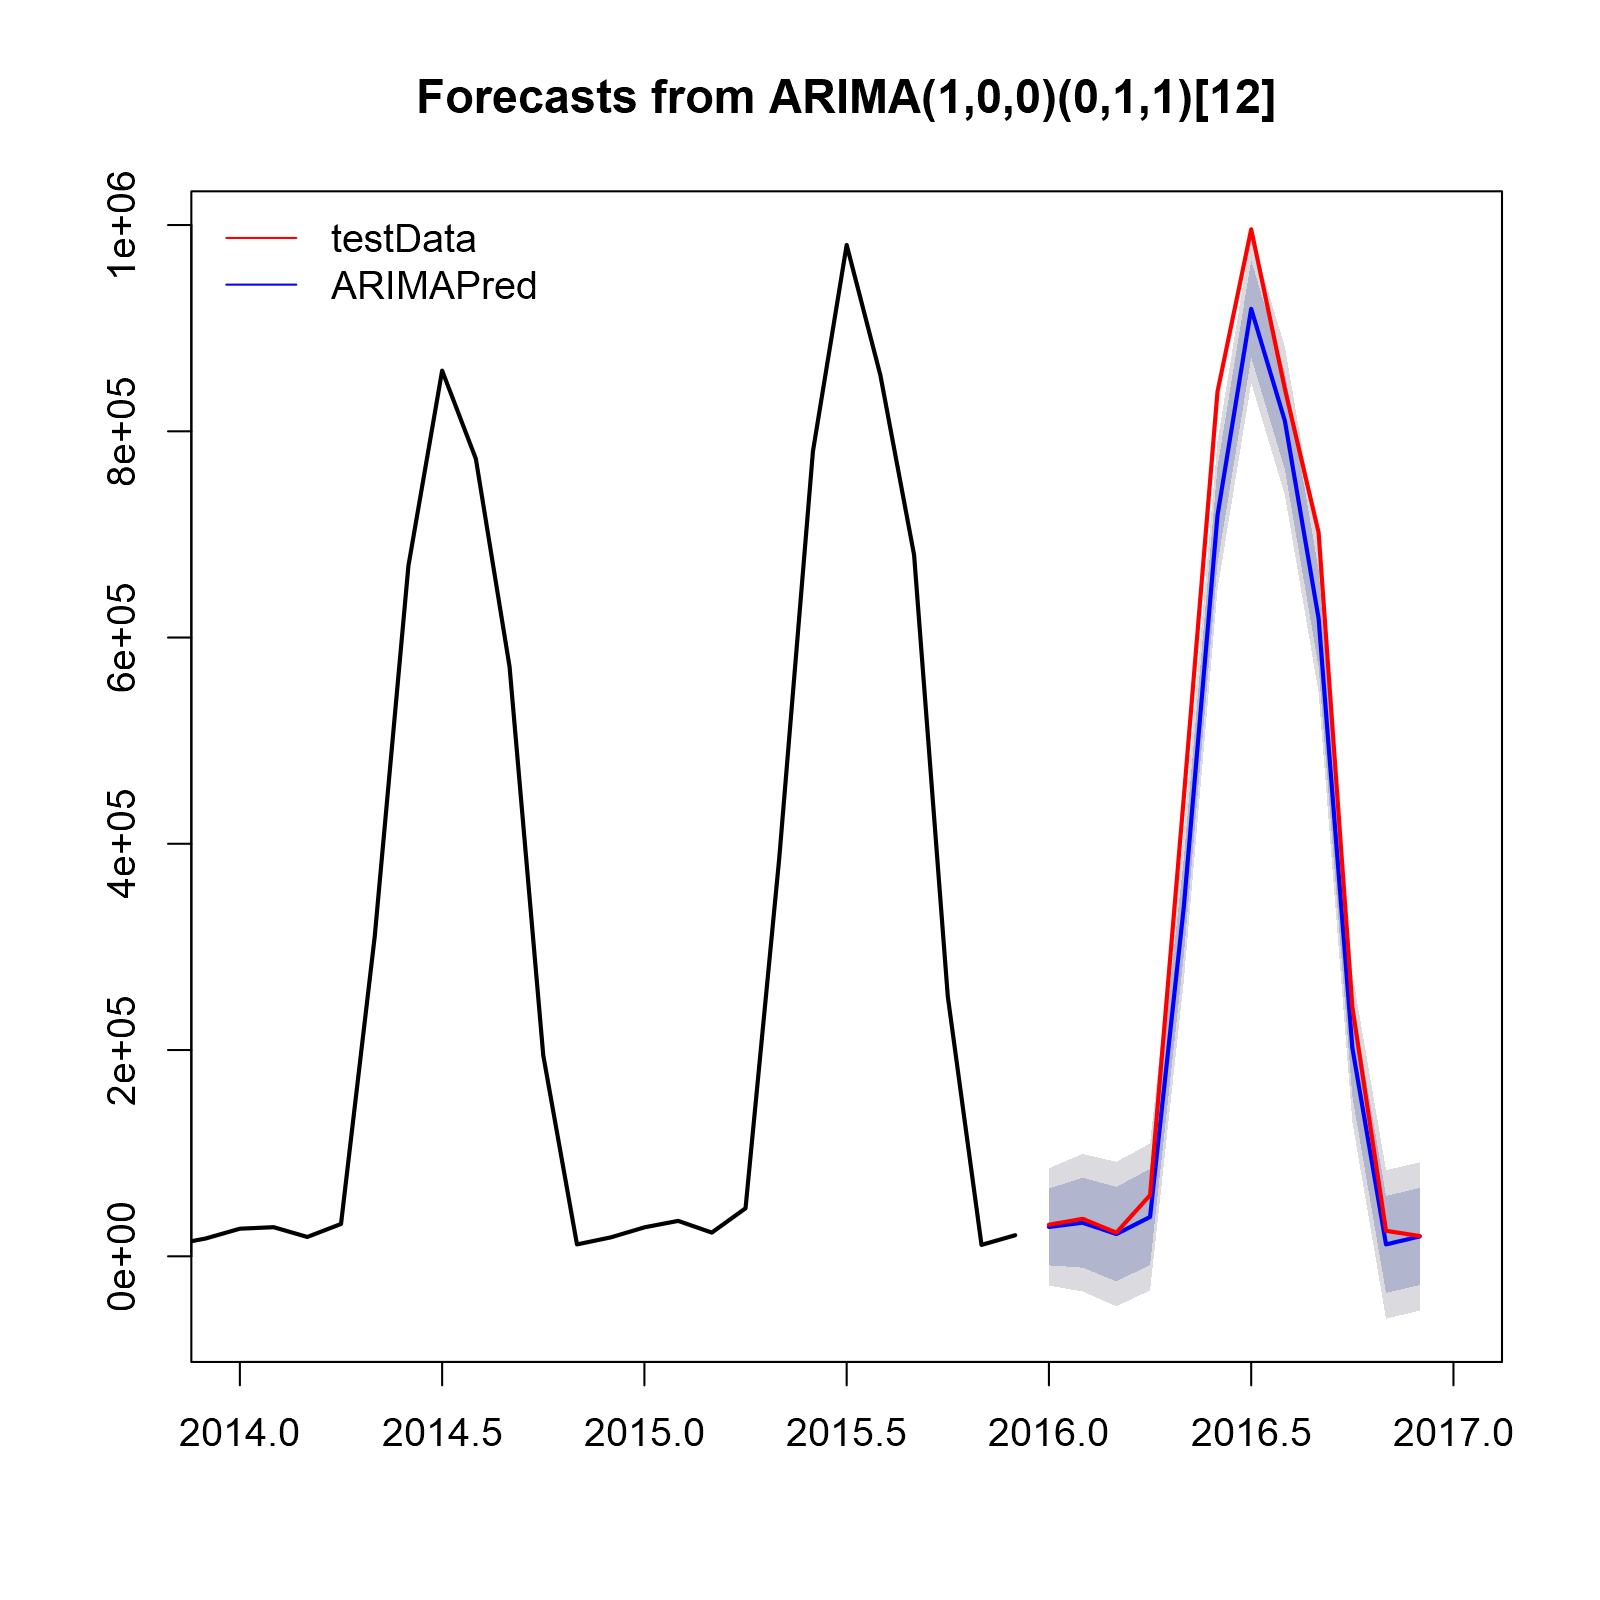
\includegraphics[width=.47\linewidth]{../normalplots/forecastGOOD-fitV-plot.png} \hfill \centering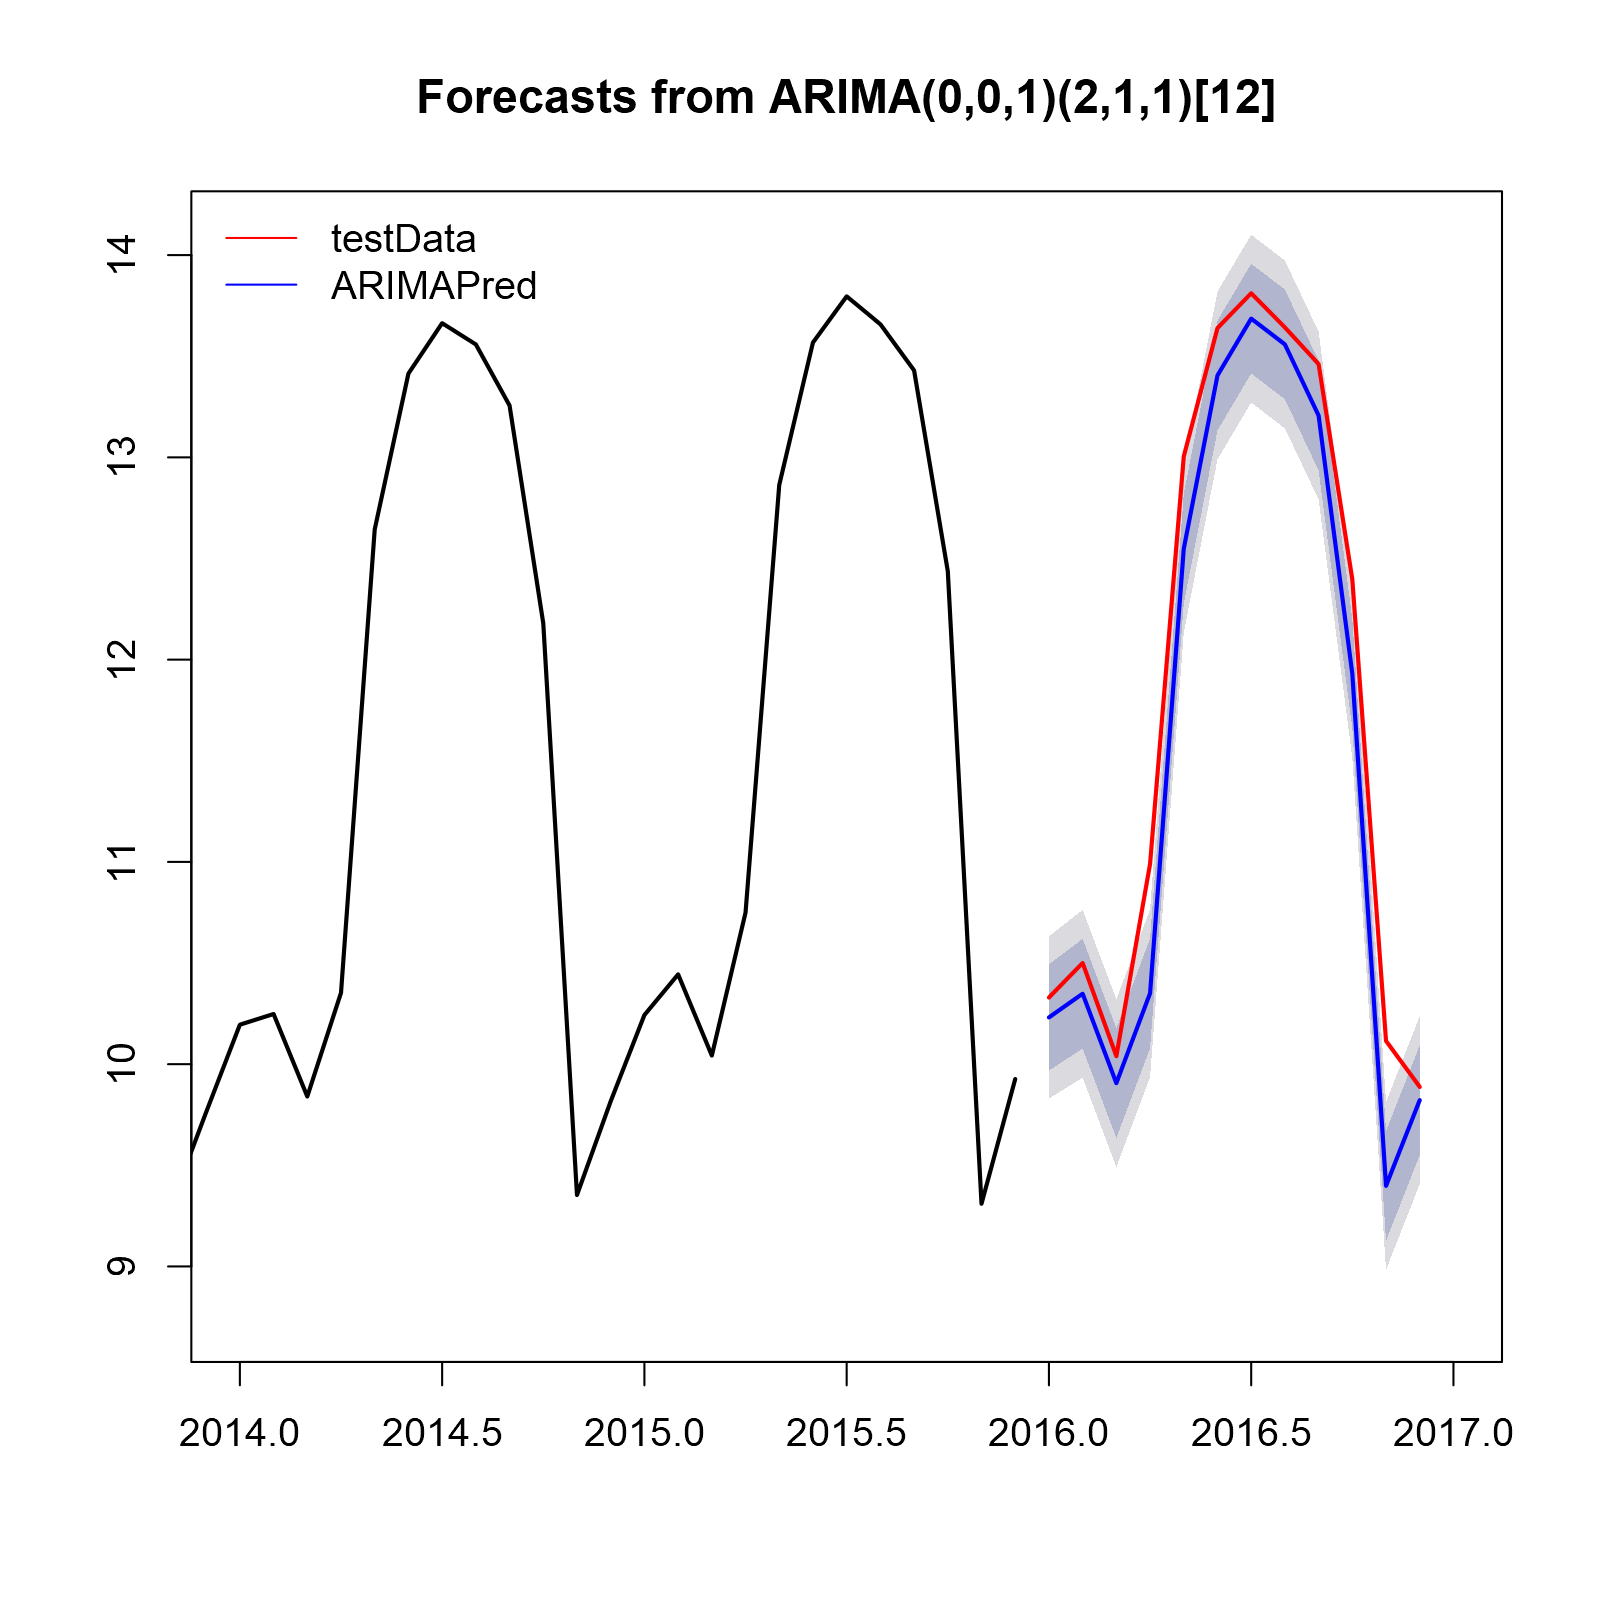
\includegraphics[width=.47\linewidth]{../normalplots/forecastGOOD-fitLV-plot.png}
\end{figure}

\vfill 
\footnotesize We again see that the non-log transformed model has a lower U value of 0.2662 than the log transformed model’s U value of 0.3558. 
\end{frame}


\section{Accounting for Outliers}
\subsection{}

\begin{frame}{1988 Wildfire}
Yellowstone fires of 1988 collectively formed the largest wildfire in the recorded history of Yellowstone National Park in the United States.

\begin{figure}
\centering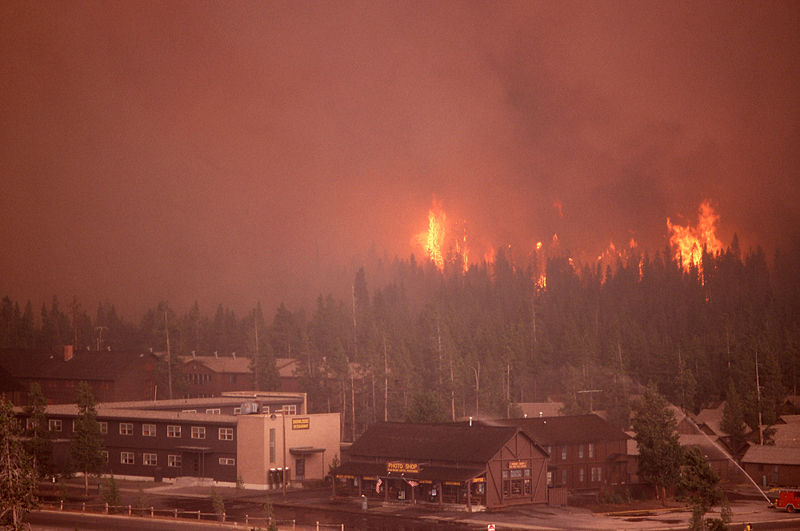
\includegraphics[width=.7\linewidth]{ysnpfire.jpg}
\captionsetup{labelformat=empty}
\caption{Fires approach the Old Faithful Complex on September 7, 1988}
\end{figure}
\end{frame}

\begin{frame}{Decomposition after replacing 1988 with 5 year average}
\small{\textbf{Regular data}\hfill \textbf{Log transformation}}
\vspace{-1em}
\begin{figure}
\centering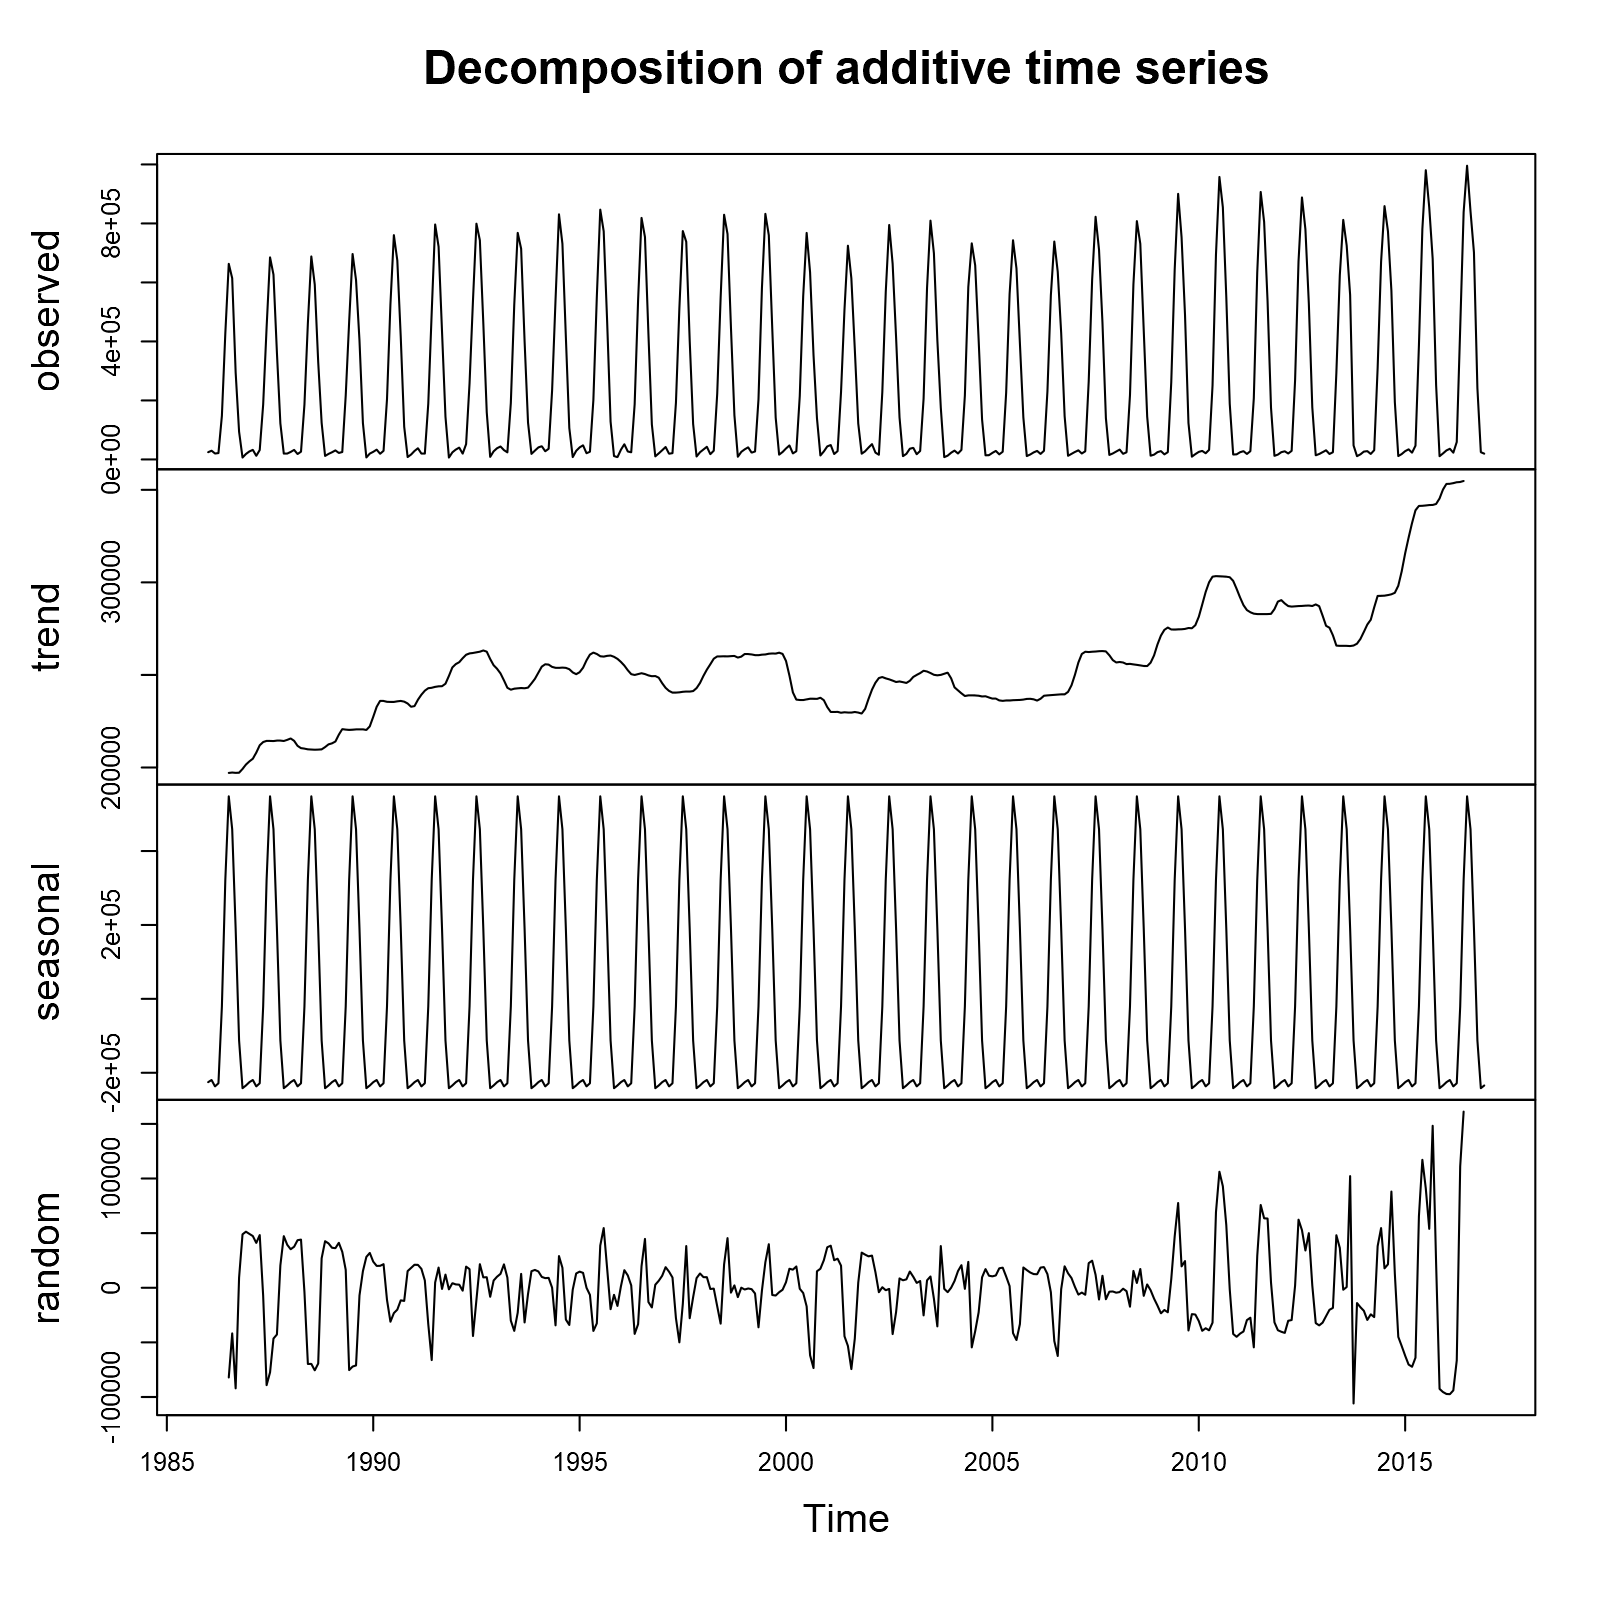
\includegraphics[width=.42\linewidth]{../outlier/visits-components-ts-plot-outlier.png} \hfill \centering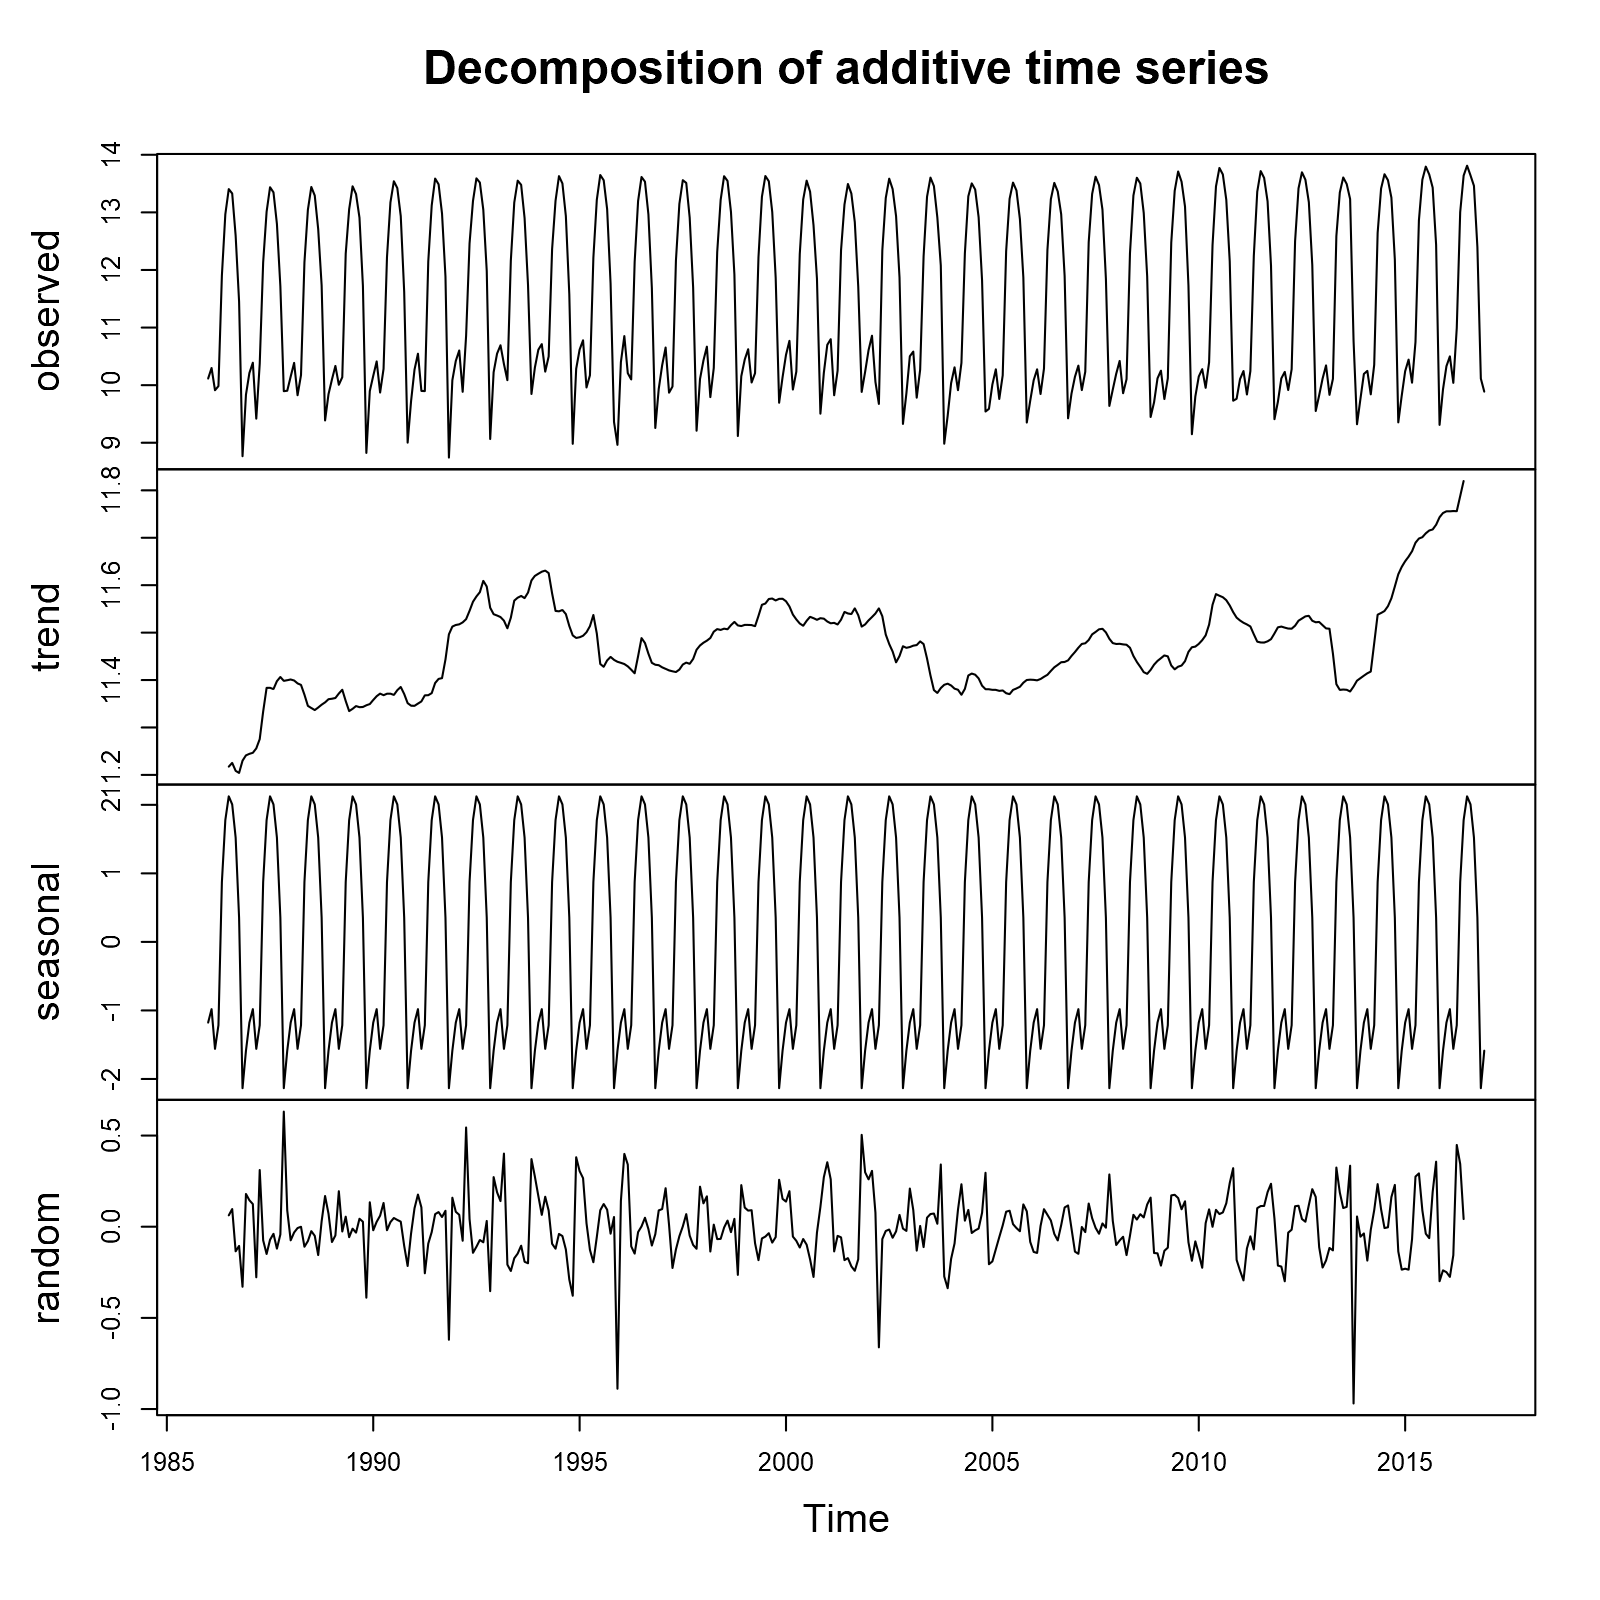
\includegraphics[width=.42\linewidth]{../outlier/Logvisits-ts-plot-outlier.png}
\end{figure}

\vfill 
\footnotesize The data manipulation fixed the outlier, and the log transforms still lessens the linear trend and decreases variance of the random errors. 
%\footnotesize It should be noted that the decomposition of the log transformed data set without outliers, that the increased variance in residuals is lessened, which is one of the reasons we still pursue the log transformation.  Also, both series passed the Augmented Dickey-Fuller Test and can be considered stationary. 
\end{frame}

\begin{frame}{New model fitting and diagnostics}
\small{\textbf{Model on regular data}\hfill \textbf{Model on log transformation}}
\vspace{-1em}
\begin{figure}
\centering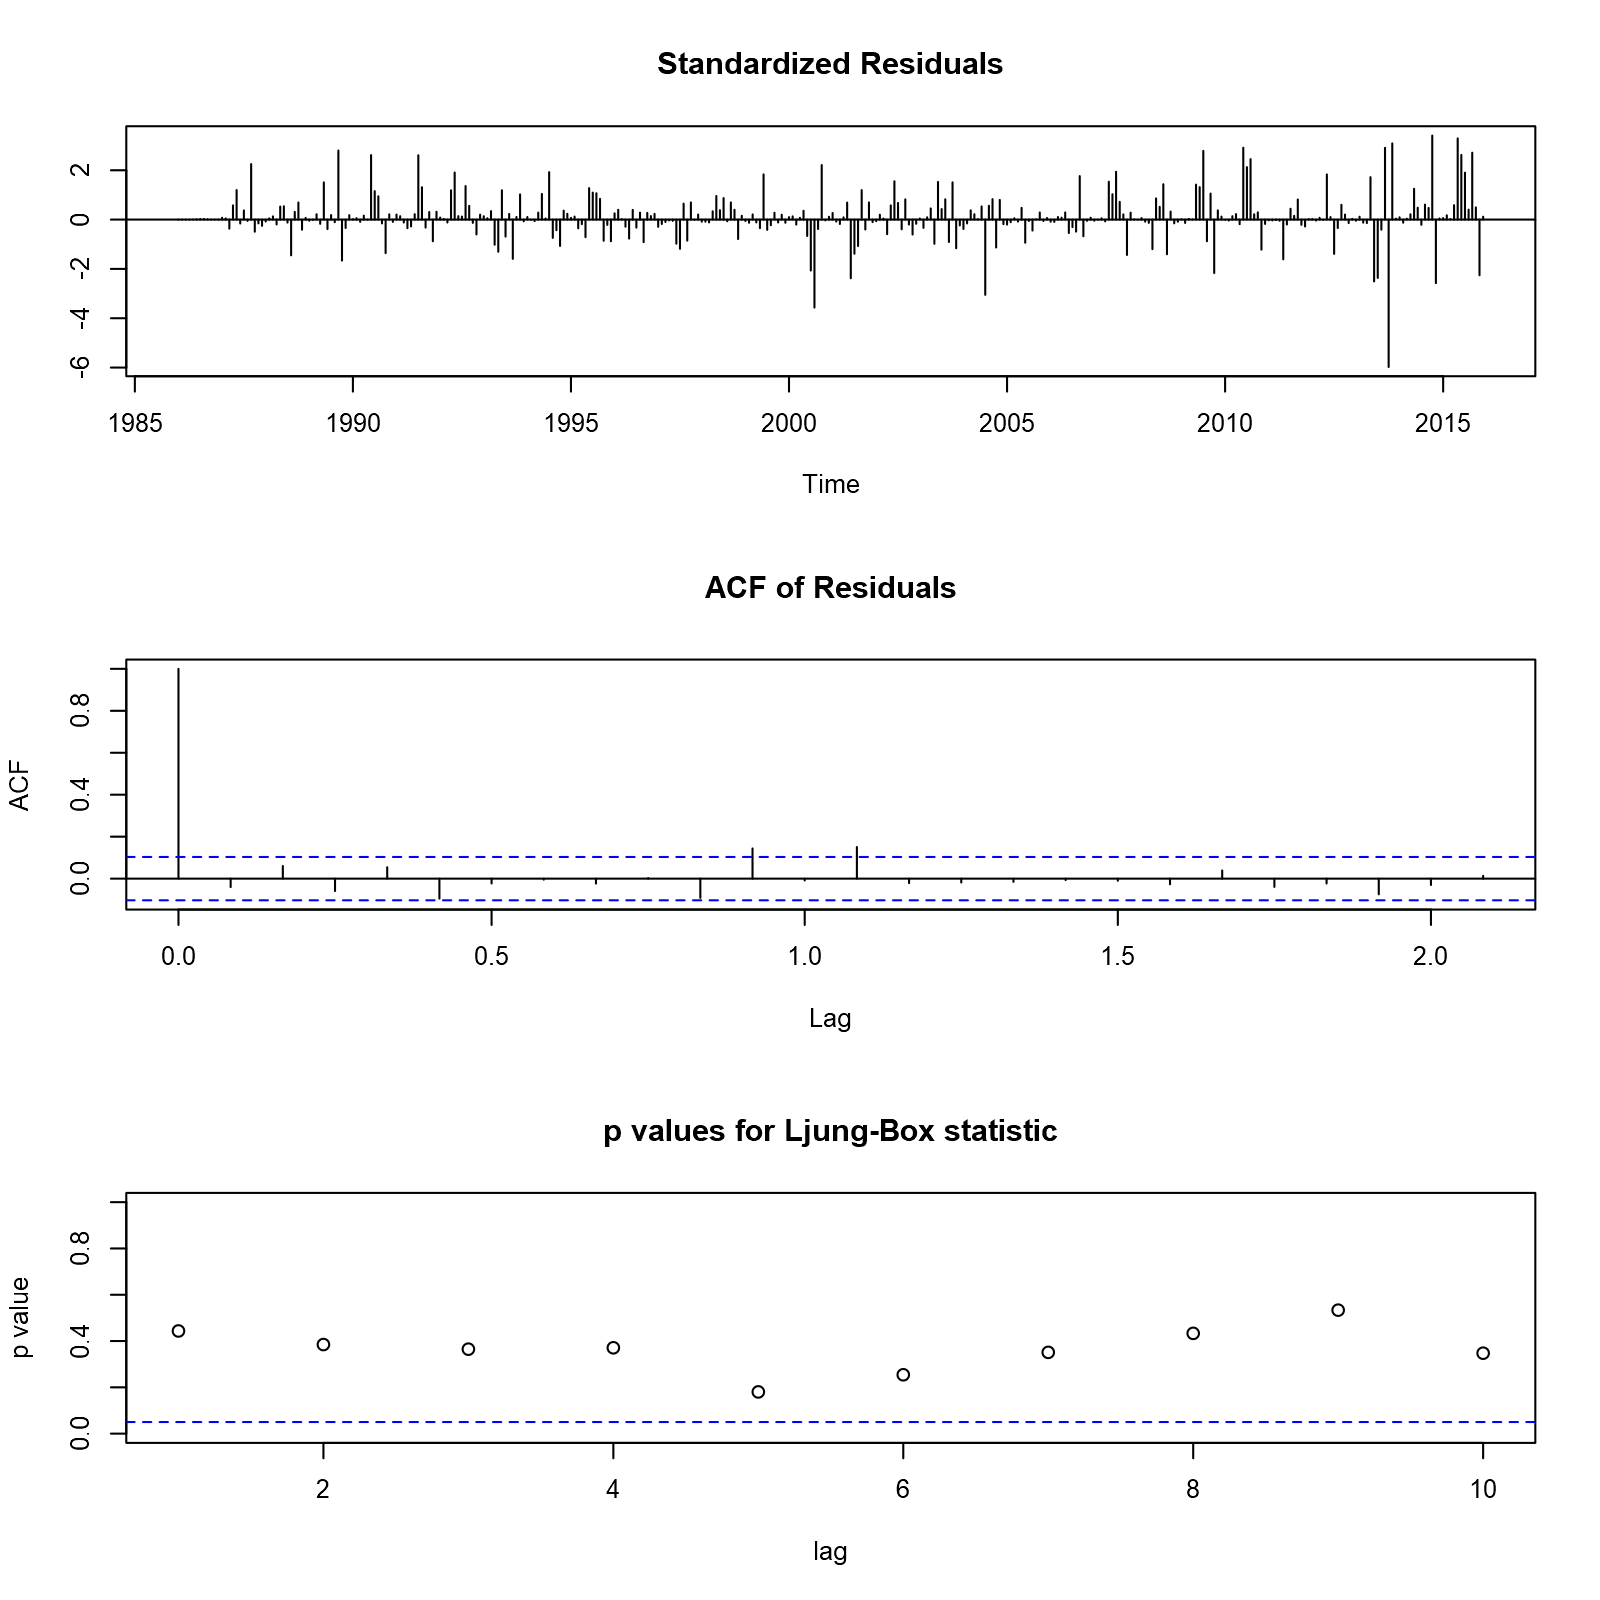
\includegraphics[width=.47\linewidth]{../outlier/tsdiag-fitV-plot-outlier.png} \hfill \centering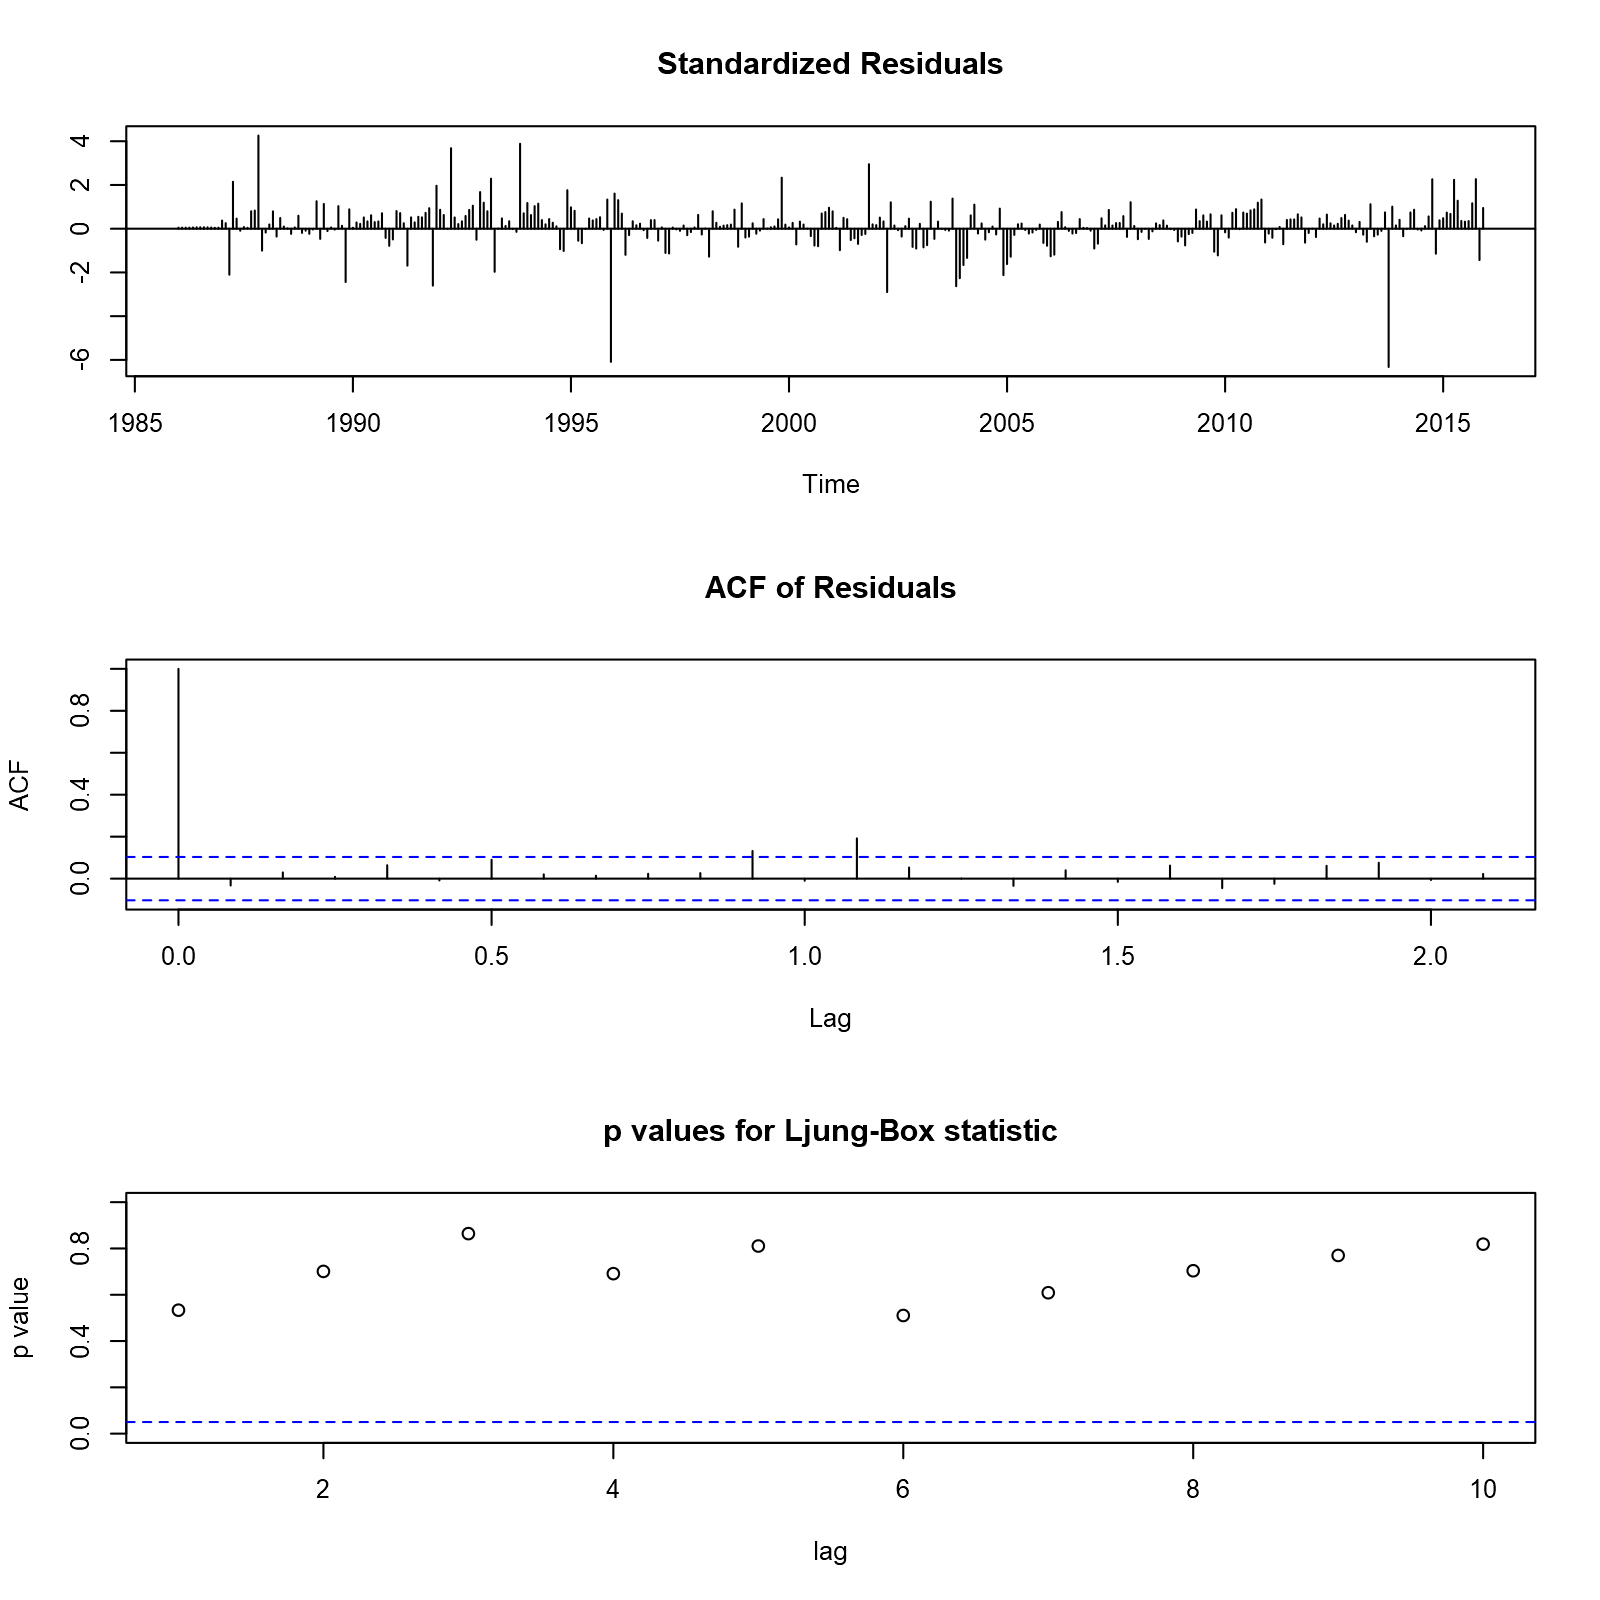
\includegraphics[width=.47\linewidth]{../outlier/tsdiag-fitLV-plot-outlier.png}
\end{figure}

\vfill 
\footnotesize The original data only has a larger outlier at 2014 now, but the log transformed data as a couple outliers.  
\end{frame}


\begin{frame}{Forecasting with the new models}
\small{\textbf{Model on regular data}\hfill \textbf{Model on log transformation}}
\vspace{-1em}
\begin{figure}
\centering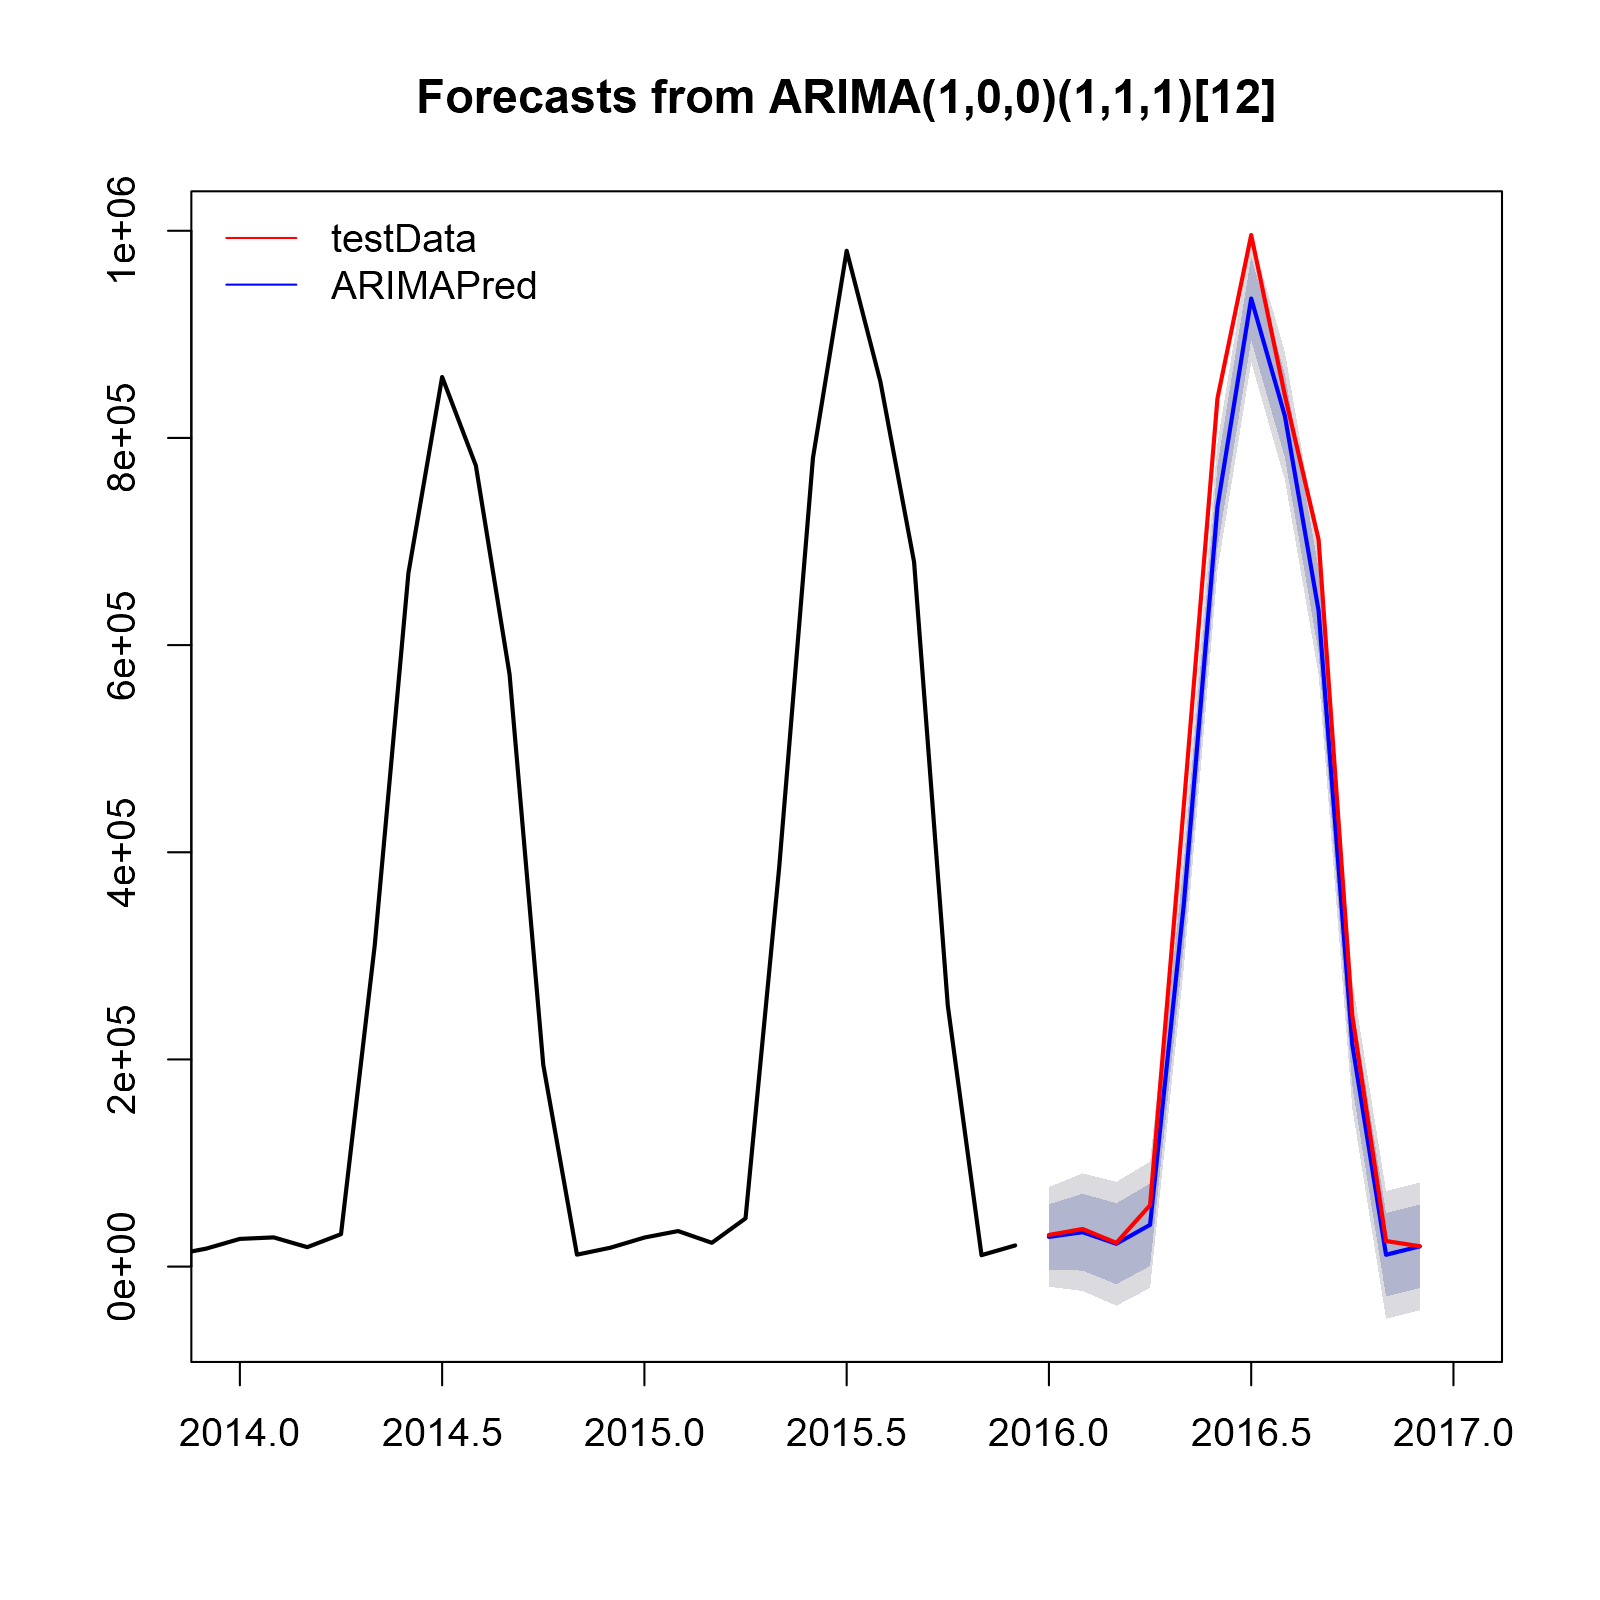
\includegraphics[width=.47\linewidth]{../outlier/forecastGOOD-fitV-plot-outlier.png} \hfill \centering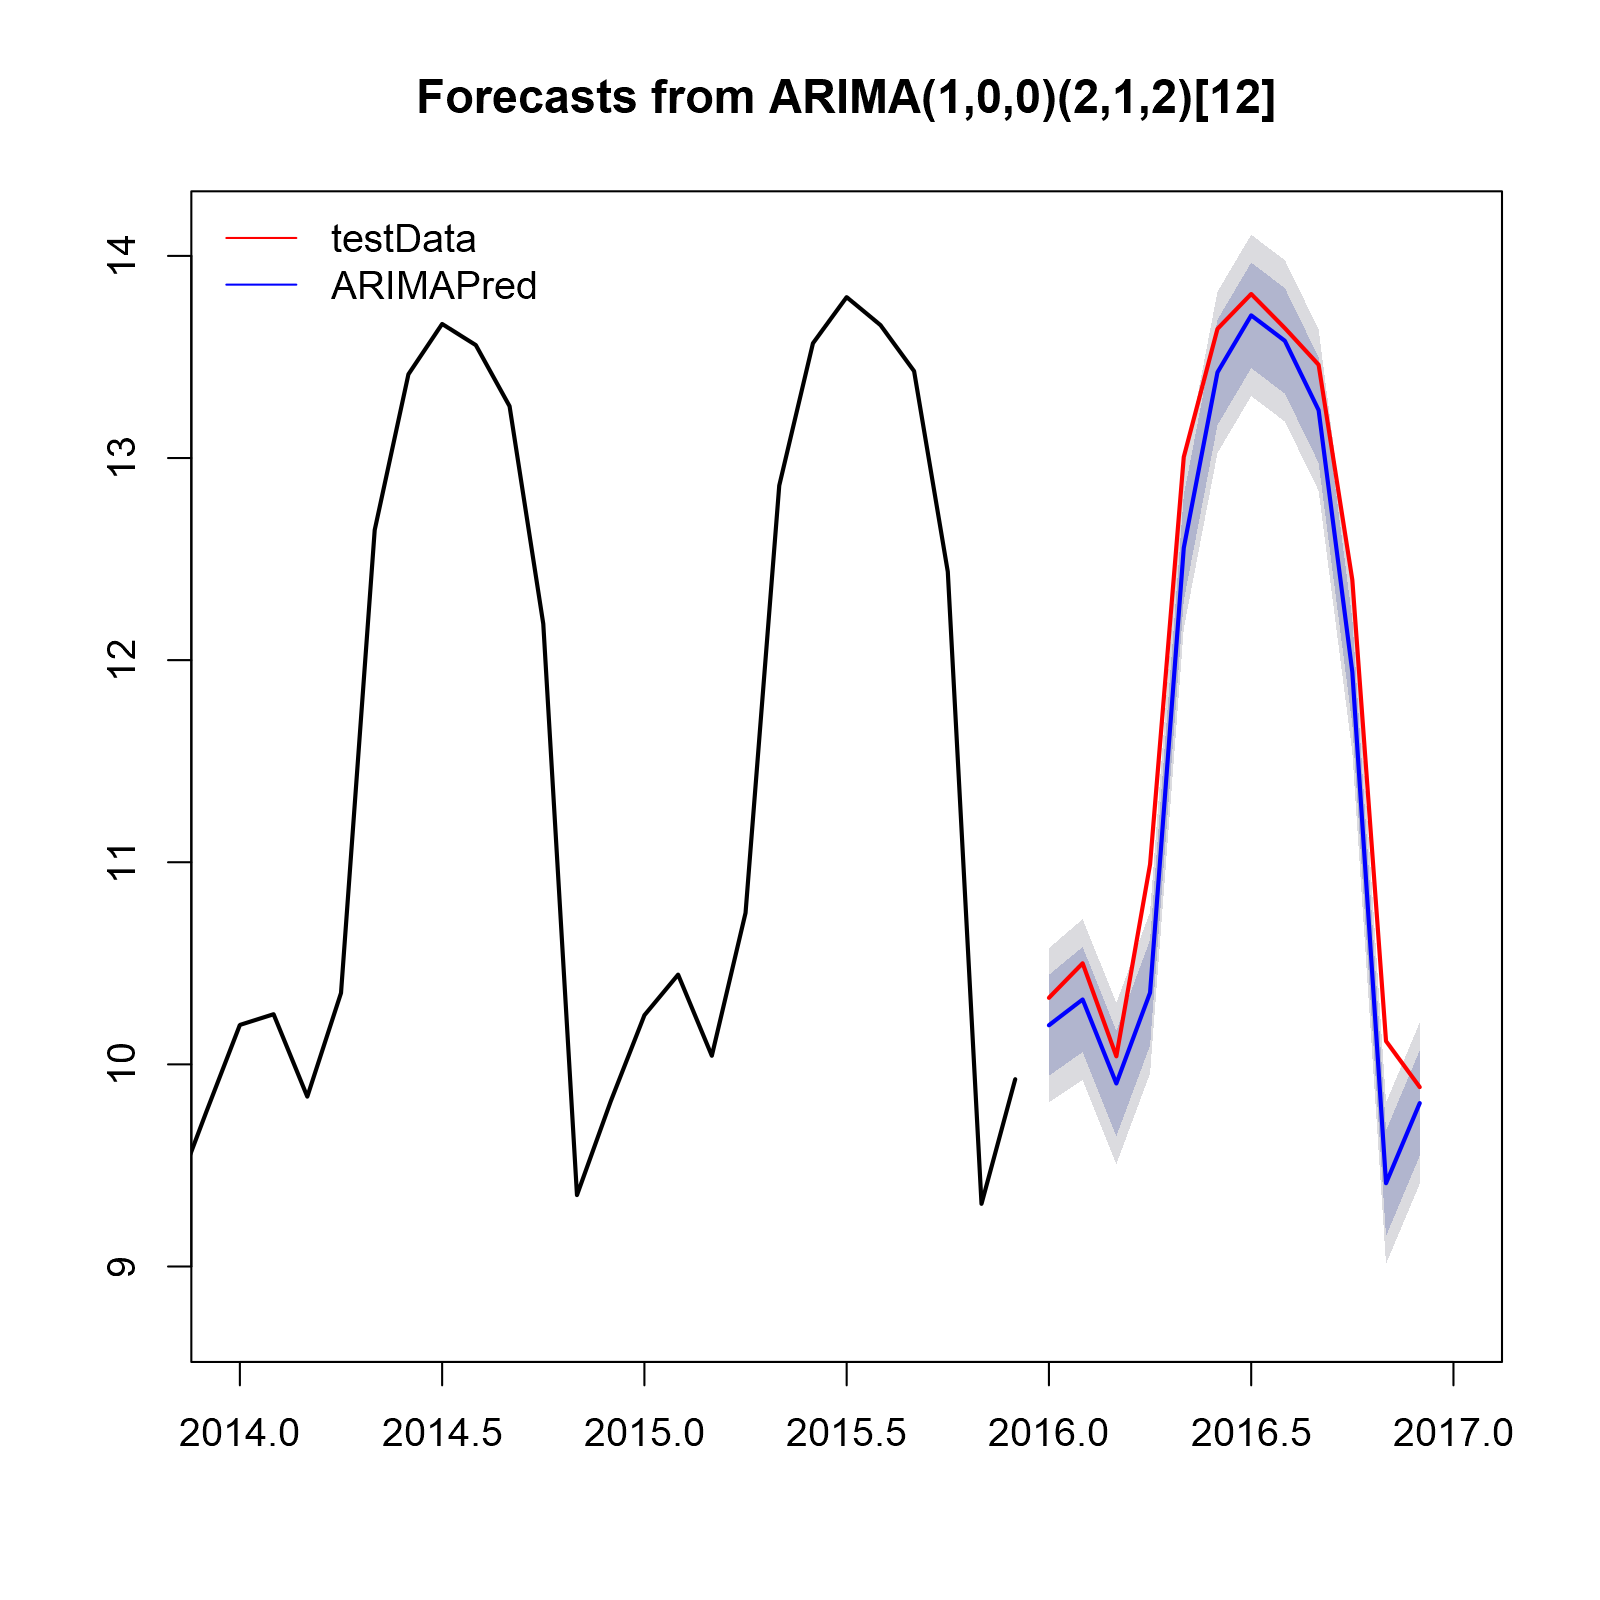
\includegraphics[width=.47\linewidth]{../outlier/forecastGOOD-fitLV-plot-outlier.png}
\end{figure}

\vfill 
\footnotesize We again see that the non-log transformed model has a lower U value of 0.2662 than the log transformed model’s U value of 0.3558. 
\end{frame}

\section{End}

\subsection{}
\begin{frame}{Conclusion}
\begin{itemize}
\item We first presented two stationary time models and found that found that  ARIMA (1,0,0) X (0,1,1) model was best suited for forecasting.  
\item We provided justification of the used of a seasonal model as well as explore some model diagnostics for what we presented. 
\item After manipulating our data to account for our largest outlier, we concluded the best model for forecasting is the ARIMA(1,0,0) X (1,1,1) with the modification of the fire year average to replace the 1988 visitor attendance because of the large wildfire.  
\end{itemize}
\end{frame}


%\begin{frame}{Experimental Design}
%
%\begin{center}
%\resizebox{\linewidth}{!}{
% \begin{tabular}{||l | l  c  c||} 
% \hline
%Scenarios & Climate & Fire & Human Response \\ [0.5ex] 
% \hline\hline
% Historic Climate & \color{recentTrends}Historic Climate & Inactive & Inactive \\ 
% \hline
% Historic Climate \& Fire  & \color{recentTrends}Historic Climate & \color{activeGreen}Active & Inactive \\
% \hline
% Historic Climate \& LU & \color{recentTrends}Historic Climate & \color{activeGreen}Active & \color{activeGreen}Active \\
% \hline
% Climate Change & \color{climateChange}Climate Change & Inactive & Inactive \\
% \hline
% Climate Change \& Fire & \color{climateChange}Climate Change & \color{activeGreen}Active & Inactive \\ 
% \hline
% Climate Change \& LU  & \color{climateChange}Climate Change & \color{activeGreen}Active & \color{activeGreen}Active \\ 
% \hline
%\end{tabular}}
%\end{center}
%\end{frame}


\end{document}


